In this chapter, we attempt the task of denoising \gls{MPES} data, beginning with an exploration of the various \gls{MPES} datasets used in this study, which include \gls{GrIr}, \gls{NiW}, \gls{GdW} and \gls{WSe2}, and examinining the characteristics relevant to analyzing the denoising performance.

Given its high electron counts, the \gls{GrIr} dataset serves as our primary reference, providing a robust target for generating higher quality (compared to other datasets) target images. This dataset forms the basis for training a deep learning model (\cref{ch:deep_learning}), while \gls{WSe2}, captured with a different experimental setup, serves as a key comparator to evaluate the generalization of denoising approaches across datasets and statistical differences due to the light sources (\cref{ch:pes-statistics}).\todo{If WSe2 is not used for denoising, remove that part.}

An overview of the data reduction and image formation pipeline is provided, illustrating how single-event data from these experiments are transformed into multidimensional images suitable for analysis. We detail how the target and noisy realizations of the data are constructed, generating representations for high-count reference images and low-count noisy images that reflect realistic experimental conditions, respectively.

In order to evaluate the performance of denoising algorithms on \gls{MPES} data, we present here the criteria and metrics used; in particular, focusing on perceptual metrics like the \gls{MSSSIM} (\cref{eq:msssim})\todo[disable]{Insert a reference to where you define this.}, which is more robust to the inherent noise in experimental reference images.

We apply the \gls{BM3D} algorithm, both with and without application of the Anscombe \gls{VST} to the \gls{GrIr} dataset, containing the highest total electron counts \gls{ncounts}. A hyperparameter search is performed to identify the optimal denoising parameters, specifically the choice of the $\sigma$ value, for different \gls{ncounts}. An evaluation of the denoising performance using the \gls{BM3D} algorithm is then demonstrated, as it has the highest counts to form an proper evaluation. This is proceeded with a discussion on the effectiveness of \gls{BM3D} in improving image quality at various count levels and the effect of applying \gls{VST} on denoising performance.

\todo[disable]{By saying that you do this one ``one'' of the data sets, you implicitly stress that you don't do it on all, so the reader will wonder why. Depending on why you only do this on one dataset, you could make this clear by adding some clarification, i.e., just the ``exemplarily'' could be enough.}

\section{Experimental Datasets}\label{section:datasets}
We investigate three datasets--\gls{GrIr} \cite{heberMultispectralTimeresolvedEnergy2022}, \gls{NiW} \cite{shokeenRealtimeObservationNonequilibrium2024}, and \gls{GdW} \cite{kutnyakhovMultidimensionalPhotoemissionSpectra2024}--that have been studied using \gls{HEXTOF} at \gls{FLASH}. Interpretable results from these experiments require long acquisition times (\gls{total_time}), essential for capturing the underlying physical processes. This is primarily due to three reasons:\todo[disable]{``that will be described below''?}

\todo[disable]{You could reference the corresponding section here}The intrinsic stochastic nature of the photoemission process requires the collection of a large number of events to approach the true value (\cref{section:photoemission-process}). Additionally, the low repetition rate and intentionally reduced flux\footnote{To mitigate the space-charge effect} of the \gls{FEL} means that the data  needs to be collected over a long period of time to get sufficient statistics (\cref{section:fel}). For example, as shown in \cref{fig:acq-time-1M}, acquiring $\num{e6}$ electron events (\gls{ncounts}) \todo[disable]{electrons? events?} requires an acquisition time of $\gls{total_time}=\qty{8}{\min}$. Lastly, the multidimensional acquisition scheme to simultaneously resolve \gls{kx}, \gls{ky}, \gls{kz}, \gls{E}, \gls{tpp}, and spin polarization necessitates exponentially \todo[disable]{You mean this scale exponentially in the number od dimensions?} more data, as the number of dimensions increases, to adequately fill the sample space in higher dimensions (\cref{section:spectroscopy-techniques}).

\begin{figure}[h]
    \centering
    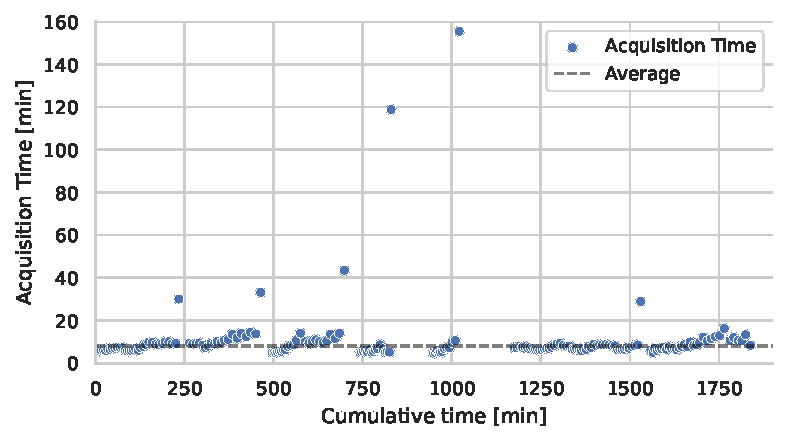
\includegraphics[width=0.8\linewidth]{images/acq_time_1M.pdf}
    \caption{Total acquisition time \gls{total_time} in minutes for generating \num{e6} data points. Some outliers are present due to the photon source being off, leading to longer \gls{total_time}. The average \gls{total_time} without outliers is approximately \qty{8}{min} (see dashed line).}
    \label{fig:acq-time-1M}
\end{figure}

For most of this study, we use the \gls{GrIr} dataset, as it features the longest acquisition time $T=\qty{30}{h}$, and hence the highest number of counts, with $\gls{ncounts}=\num{1.86e8}$\todo[disable]{You may also want to (re-)state $T$ for this data set here.}. The \gls{NiW} and \gls{GdW} datasets have comparatively lower total counts, at $\gls{ncounts}$ of \num{6.52e7} and \num{2.21e7}, respectively. 

However, \gls{ncounts} is not the only factor in determining data quality. Material-specific factors, sample conditions, and instrument settings can influence spectral clarity, meaning that a higher-count dataset does not necessarily guarantee more pronounced spectral features. For instance, while the \gls{NiW} dataset has higher counts \todo[disable]{Why ``\gls{ncounts}''? Isn't this the number of counts that you are referring to? I would interpret ``rate'' as counts per time, but you seem to give the absolute counts here.}\tododone[disable]{Yes, just by mistake} than \gls{GdW}, its spectral features are comparatively less distinct as seen in \cref{fig:all-hextof-datasets-kxky}.

\begin{figure}[h]
    \centering
    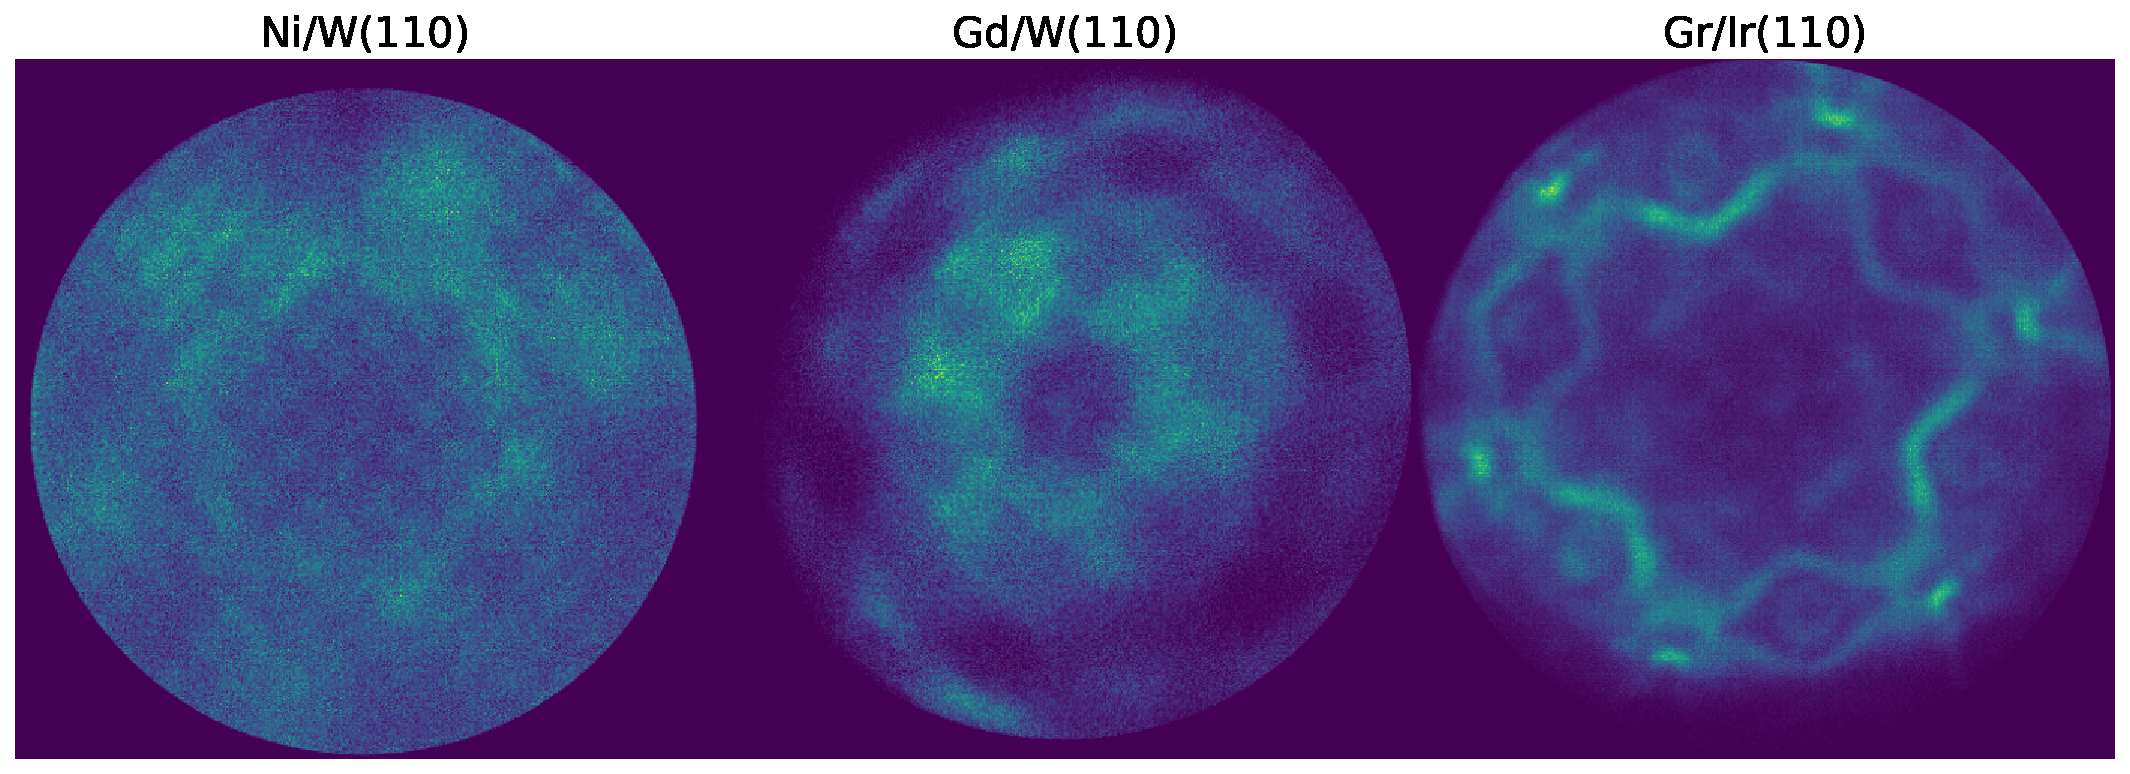
\includegraphics[width=1\linewidth]{images/datasets_3_kx_ky.pdf}
    \caption{A \gls{kx}-\gls{ky} slice of the \gls{GrIr}, \gls{NiW}, and \gls{GdW} datasets, slice summed across \gls{E} with size \todo[disable]{insert ``window size''}$\gls{winsize}=\num{20}$\todo[disable]{Is the size in ``bins''? I guess what this means will only become clear in Section 4.2. If this is the case, you also can reference this here, so the reader will know to look for the details furher down.}. See \cref{sec:image-formation} for details on how these images are formed.}
    \label{fig:all-hextof-datasets-kxky}
\end{figure}

For reference, we also look at the \gls{WSe2} dataset \cite{maklarTimeresolvedARPESRAW2022}, measured with a pulsed \gls{HHG}-based \gls{XUV} source using a \gls{TOF}-\gls{MM} analyzer\footnote{The \gls{TOF}-\gls{MM} analyzer being the common aspect between the \gls{GrIr} etc./ and the \gls{WSe2} dataset.} and a single-segmented \gls{DLD}. This setup yields a significantly larger number of counts, recording $\gls{ncounts}=\num{1e9}$ within $\gls{total_time}=\qty{27}{s}$. In comparison, the \gls{GrIr} dataset, collected with a \gls{FEL} source, yields $\gls{ncounts} = \num{1e6}$ over $\gls{total_time} = \qty{8}{\min}$, thus producing about four orders of magnitude fewer events.

A direct denoising comparison between these datasets, however, is not feasible due to fundamental differences in light sources and detector design. The \gls{WSe2} dataset was acquired with a single-segmented detector setup, whereas the \gls{GrIr} dataset employed a more complex 8-segment detector (\cref{section:8s-dld}) that offers enhanced multi-hit capability through overlapping segments, but impacting count statistics. This already implies that the finding equivalent noise levels between the datasets is a non-trivial task.

Additionally, the inherent statistical properties of the light sources (\cref{section:light-sources}) impact the noise characteristics in the raw data. Consequently, in \cref{ch:pes-statistics}, the \gls{WSe2} dataset aids in understanding statistical differences between acquisition setups. However, direct denoising comparisons between \gls{HHG} and \gls{FEL} sources would not be meaningful due to these varied conditions and detector architectures.

\section{Data Processing and Image Formation}\label{sec:image-formation}

In an \gls{MPES} experiment using a \gls{TOF}-based scheme, the workflow to resolve images typically follows a series of steps, outlined in \cref{fig:mpes_workflow}. Prior to this, an essential step is data reduction. For the specific case of \gls{HEXTOF} instrument at \gls{FLASH}, used in our studies, a detailed description of the reduction process is outlined in Appendix~\ref{sec:elt}.

After the data reduction, corrections are applied to the measurement axes \todo[disable]{Minor cosmetic remark: Since you are not using \texttt{frenchspacing}, there is a double space after a ``.'' to mark the end of a sentence. This will also put such a double space after things like ``e.g.'' so it will look like an end of a sentence, even if it is not. One way to fix that would be to put a comma (before and) after ``e.g.'', i.e. ``, e.g.,''. Another way would be to put a backslash in front of the space after the ``.''. As I said though, this is a minor cosmetic issue, you can just ignore it if you want.} e.g.\ to correct space-charge distortions (see \cref{section:spectroscopy-techniques}), correct timing jitter between \gls{FEL} and pump laser etc. The corrected axes are then mapped (calibrated) to the physical axes, after which further correction steps can happen. Once calibrated, the single-event data is binned into a multidimensional volume\footnote{We make use of the Single Event DataFrame (SED) library \href{https://github.com/OpenCOMPES/sed}{https://github.com/OpenCOMPES/sed}.} that represents the full measurement, as illustrated on the right side of \cref{fig:mpes_workflow}.

\begin{figure}[h]
    \centering
    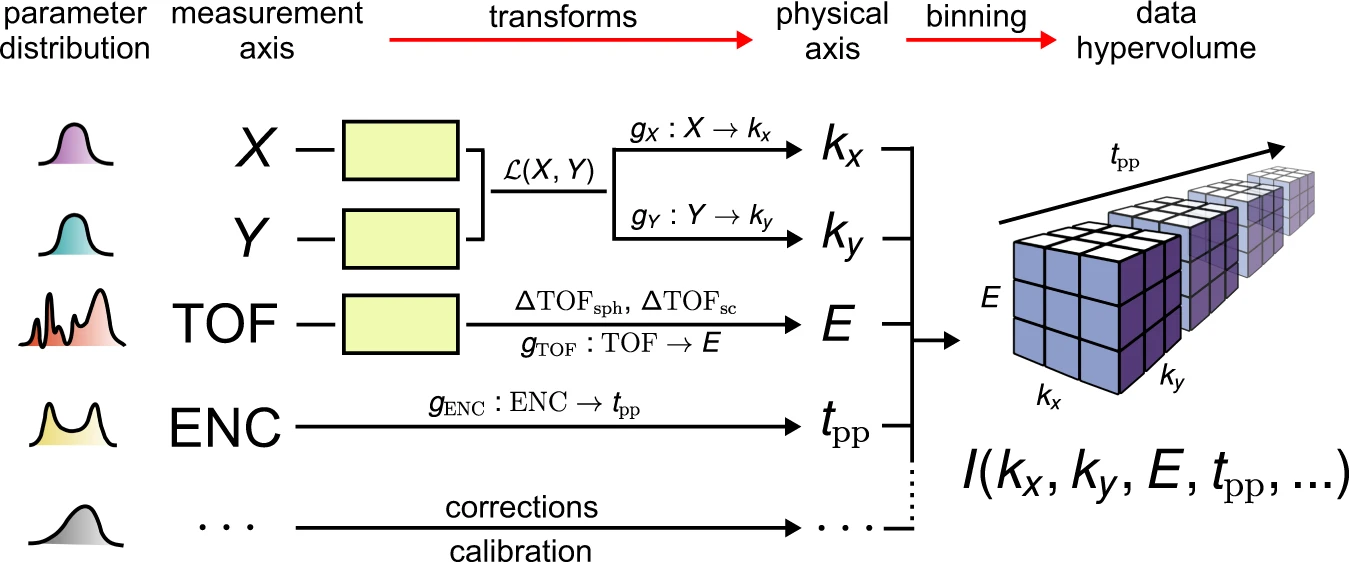
\includegraphics[width=1\linewidth]{images/41597_2020_769_Fig2_HTML.png}
    \caption{A typical workflow for an \gls{MPES} experiment, comprising transformations to the measured data and binning to form the multidimensional image. Reprinted from \cite{xianOpensourceEndtoendWorkflow2020}, under the terms of the Creative Commons Attribution 4.0 International License.}
    \label{fig:mpes_workflow}
\end{figure}

\subsection{Constructing Images from Single-Event Data}

\begin{figure}[h]
    \centering
    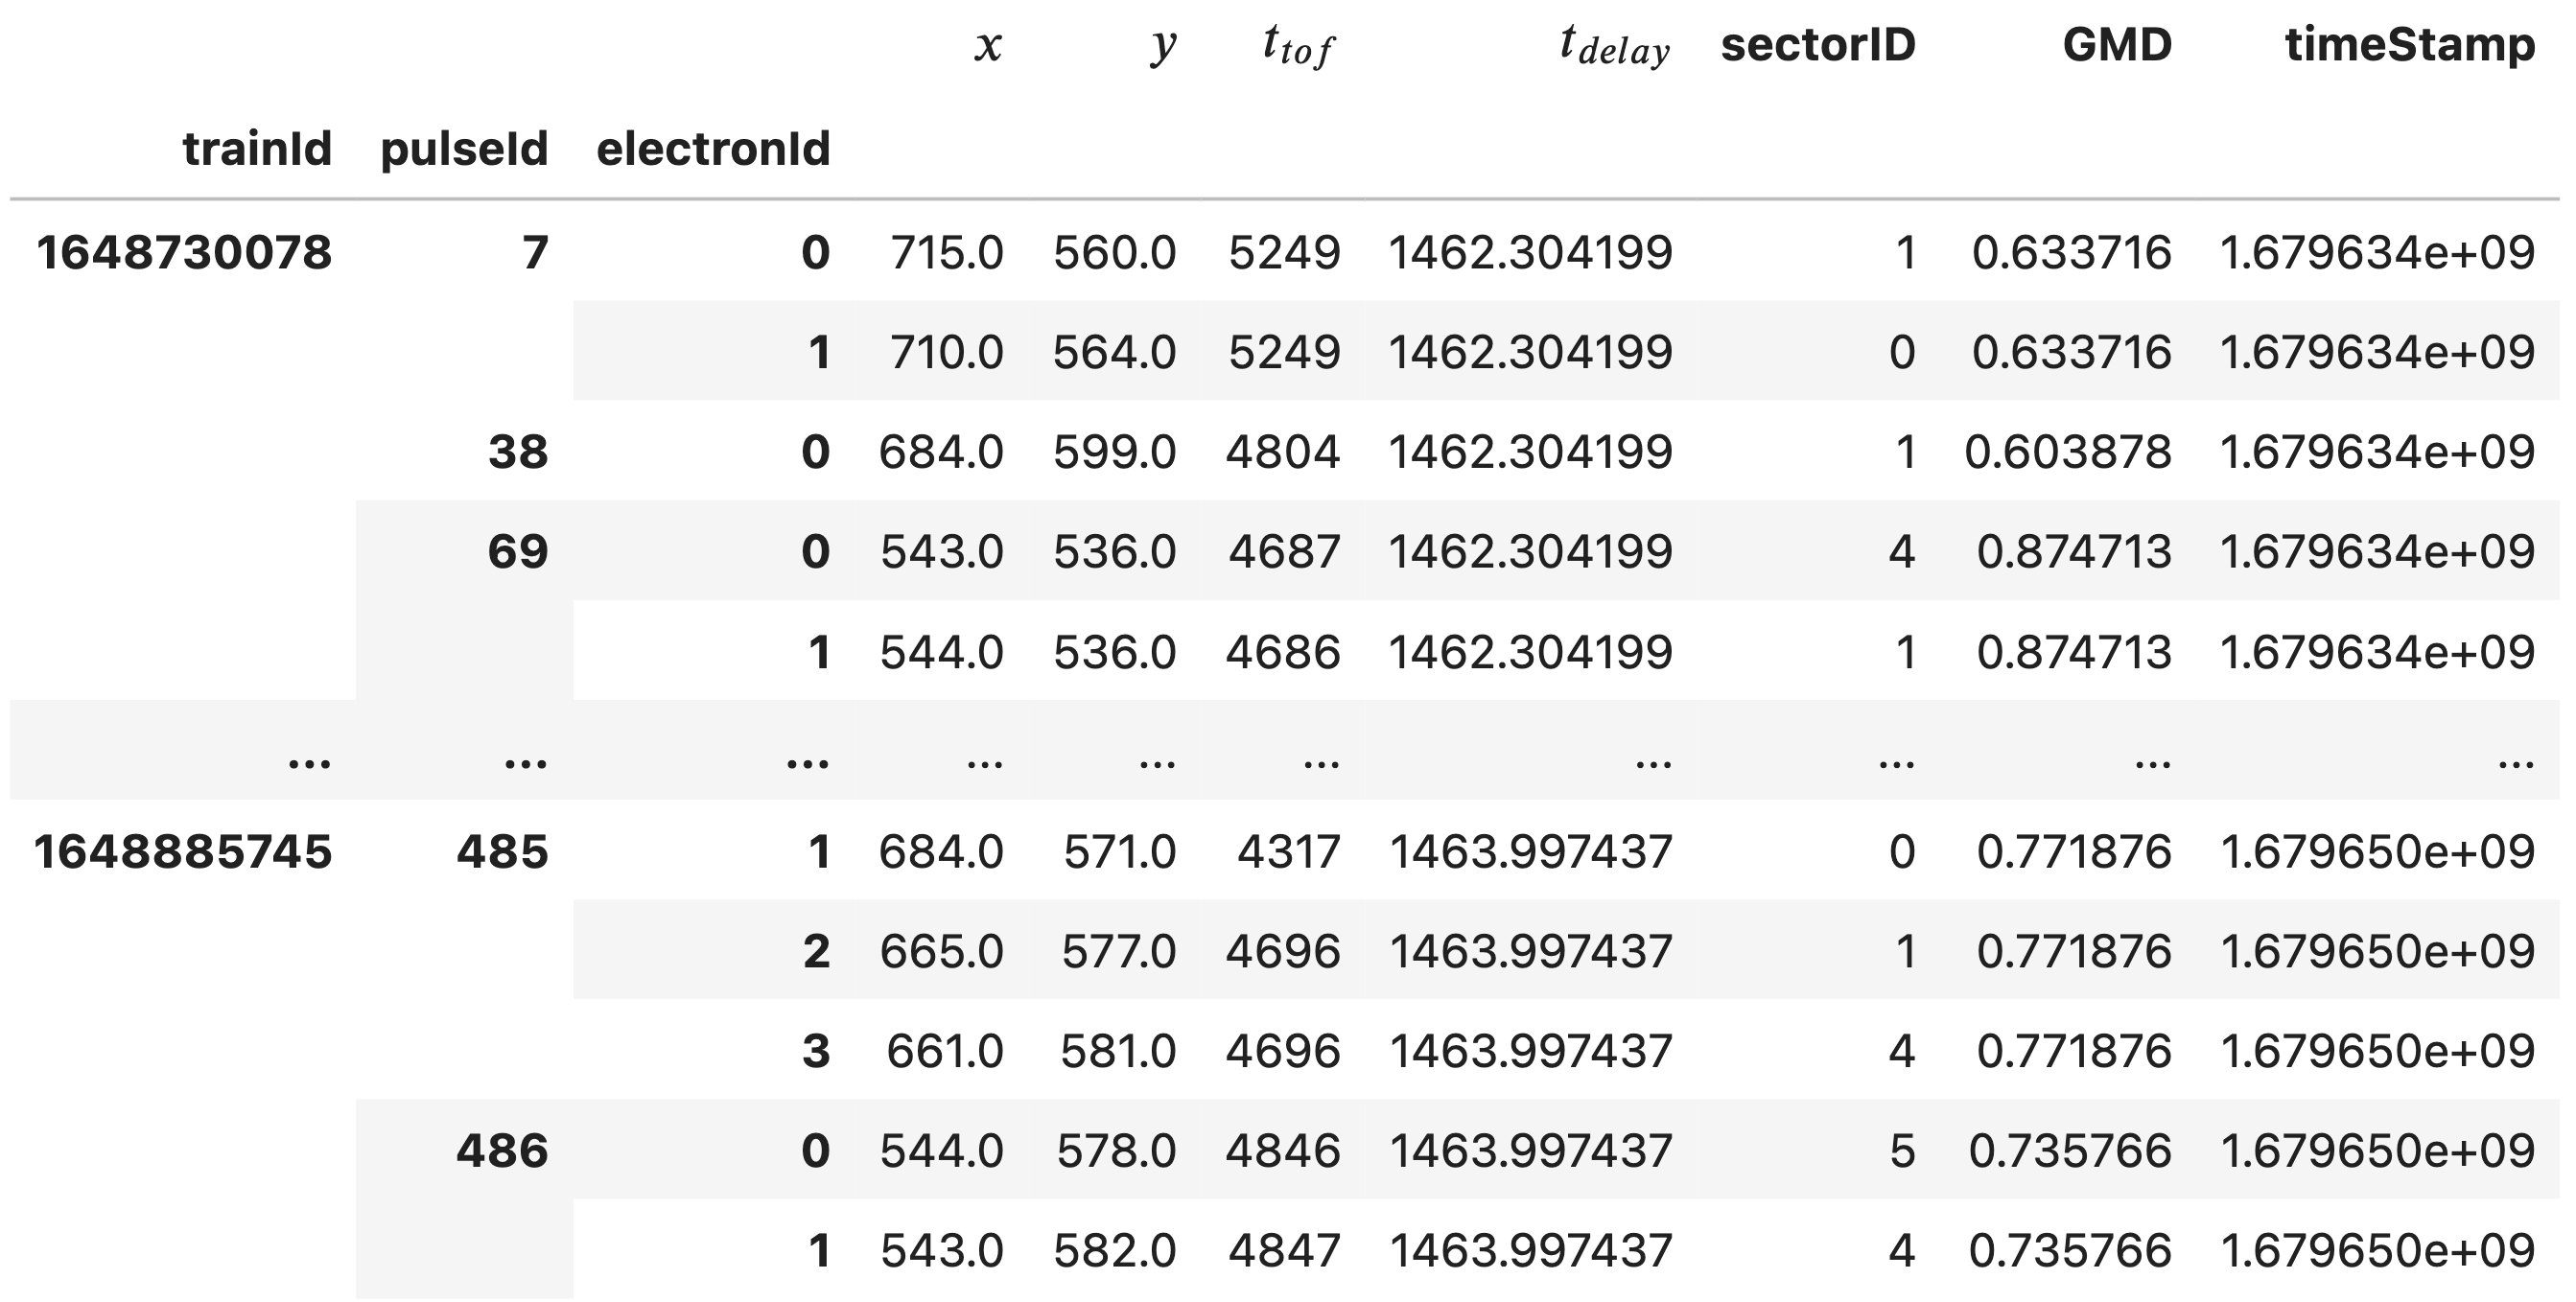
\includegraphics[width=1\linewidth]{images/dataframe.png}
    \caption{\textit{Single-event data table:} displaying the first and last five rows of recorded \gls{NiW} dataset. The table includes the detector dimensions $x$, $y$, and $t_{tof}$, which represent the spatial and time-of-flight coordinates for each detected electron (resolved at the electronId level). It also shows (unadjusted with respect to $t_0$) pump-probe delay stage values $t_{delay}$ (resolved per train), the sectorID (a unique identifier for each detector segment), the \gls{gmd} (GMD) readings (averaged per pulse), and (UNIX style) timeStamps (accurate to each train). Data is hierarchically indexed by trainId (\gls{train}), pulseId (\gls{pulse}), and electronId (event number within each pulse). Non-resolved values, such as those linked only to trains or pulses, are forward-filled for consistency across rows, allowing easy alignment with per-event data. To optimize binning and computations, certain columns can be selectively dropped to reduce dimensionality, such as when focusing on specific features like static spectra (e.g., $k_x$–$k_y$–$E$) or dynamic response data (e.g., energy $E$ vs.\ delay $t_{delay}$). Additionally, rows can be filtered to include only selected ranges, such as a particular energy interval, before the binning step.\todo[disable]{Needs better caption and reference in text}}
    \label{fig:df}
\end{figure}

In \cref{eq:images}, we defined a $d$-dimensional latent clean image $Y$ (and noisy image $X$). For most of the thesis, we focus on images with $d \in {2,3}$, as most denoising algorithms are designed to work with 2D or 3D images. Moreover, since even 3D images are commonly visualized as a series of 2D images, it is an intuitive place to begin. 

Let us hence look at how such a 3D image is constructed from the single-event data. As shown in \cref{fig:df}, the example single-event \gls{NiW} data is stored in a table format, with each row representing a single electron-event. Of physical interest are $x$, $y$, $t_{\text{tof}}$ and $t_{delay}$ that map to the physical axes \gls{kx}, \gls{ky}, \gls{E} and \gls{tpp}, respectively, where the other columns are example diagnostic and timing quantities, although they represent only a subset of the measurable quantities and diagnostics available in the experiment.

An example 2D image can be formed by selecting $t_{\text{tof}}$ and $t_{delay}$ columns and binning across these dimensions, with the image showing the dynamical energy response, or with $x$ and $y$ columns, forming a momentum image. By selecting three columns such as $x$, $y$ and $t_{\text{tof}}$, we form a 3D image as shown in \cref{fig:3d-gr-ir}.

Since the detector can capture a broad dynamic range of quantities, spanning extensive energy and momentum ranges, filtering\footnote{The range can also be reduced post binning.} is crucial to generate meaningful images. For instance, the detector records a wide range of energies, but not all are relevant to the analysis; typically, we focus on energies close to the Fermi level. 

Binning these three filtered axes forms a 3D $x$--$y$--$t_{\text{tof}}$ image. \cref{fig:3d-gr-ir} shows such images from the \gls{GrIr} dataset, with filtered energy values to be near the Fermi level \gls{EF}. Since the $t_{delay}$ axis is dropped, the dynamics are summed and this therefore, this image forms only an approximation of an image from a static momentum and energy resolved study. Nonetheless, since the dynamic effects are orders of magnitude smaller, this approximation suffices.

As physical interpretation is the goal, the general scheme is to calibrate the axes to the physical quantities first, and then bin the data to form the multidimensional image. However, in this study, we do not calibrate the data and use the detector quantization as the binning resolution, as calibrating can be non-linear in dimensions such as energy. Nonetheless, we will generally refer to the physical axes as they are conventionally used in the domain, even though we use the detector axes for binning.

Where the spatial dimensions ($x$ and $y$) are linearly mapped to the physical axes (\gls{kx}, \gls{ky}), the $E$ axis has a non-linear (quadratic) scaling with $t_{\text{tof}}$, making the $t_{\text{tof}}$ bins non-uniform in size when mapped to the $E$ axis. The non-linear scaling can potentially change the noise-profile of the data, which has potential to impact denoising performance. It is yet to be investigated if this impact has a positive or negative output, and is a potential avenue for future work.

In the aforementioned 3D images, spatial dimensions ($x$ and $y$ directions) are binned with a resolution of \qty{460}{px}, corresponding to the native detector quantization. The $t_{\text{tof}}$ is also binned with \num{460} steps to match the spatial resolution\footnote{This is done to easily form equal-resolution 2D cuts across any dimension.}. 

It is often useful to bin the data at a coarser granularity than the detector's native resolution, mainly to address low-count statistics, producing a representation that has lower resolution but higher count statistics\footnote{Where this could indeed change the noise statistics, this is a fair compromise for low-count data.}. Coarse binning can be applied to a single dimension or across multiple dimensions. For instance, \cref{fig:all-hextof-datasets-kxky} showed 2D \gls{kx}--\gls{ky} images formed by summing \num{20} slices along the $E$ axis of the 3D image. This is effectively the same as coarsely binning the $E$ axis, and selecting a single slice from this coarser 3D image. Throughout this text, we use the native detector resolution as the baseline, and for coarser analyses, we specify the slice summing size, \gls{winsize}, to define the averaging applied along a certain dimension. \todo[disable]{But this one uses additional averaging, doesn't it? Should also be mentioned here.}

While the full dataset contains \num{1.86e8} electron counts, the selected energy region used to generate the image in \cref{fig:3d-gr-ir-186M} contains \num{1.15e8} counts. Note that as discussed in \cref{section:8s-dld}, the majority of events are counted multiple times, with the most common case being that each event is recorded twice. This suggests that the effective number of counts is approximately half of \num{1.15e8}, i.e.\ \num{5.75e7}. For consistency, \gls{ncounts} is always referring to the total dataset count (\num{1.86e8} in this case), even if the actual unique counts may be lower due to multiple counting of events, or due to filtering of the energy range. This reason and a difference in detector dimensions is key reason for the difficulty in comparison of \gls{GrIr} dataset with \gls{WSe2}, which is recorded with another light source--detector setup.

\begin{figure}
    \centering
    \begin{subfigure}[t]{0.49\linewidth}
        \centering
        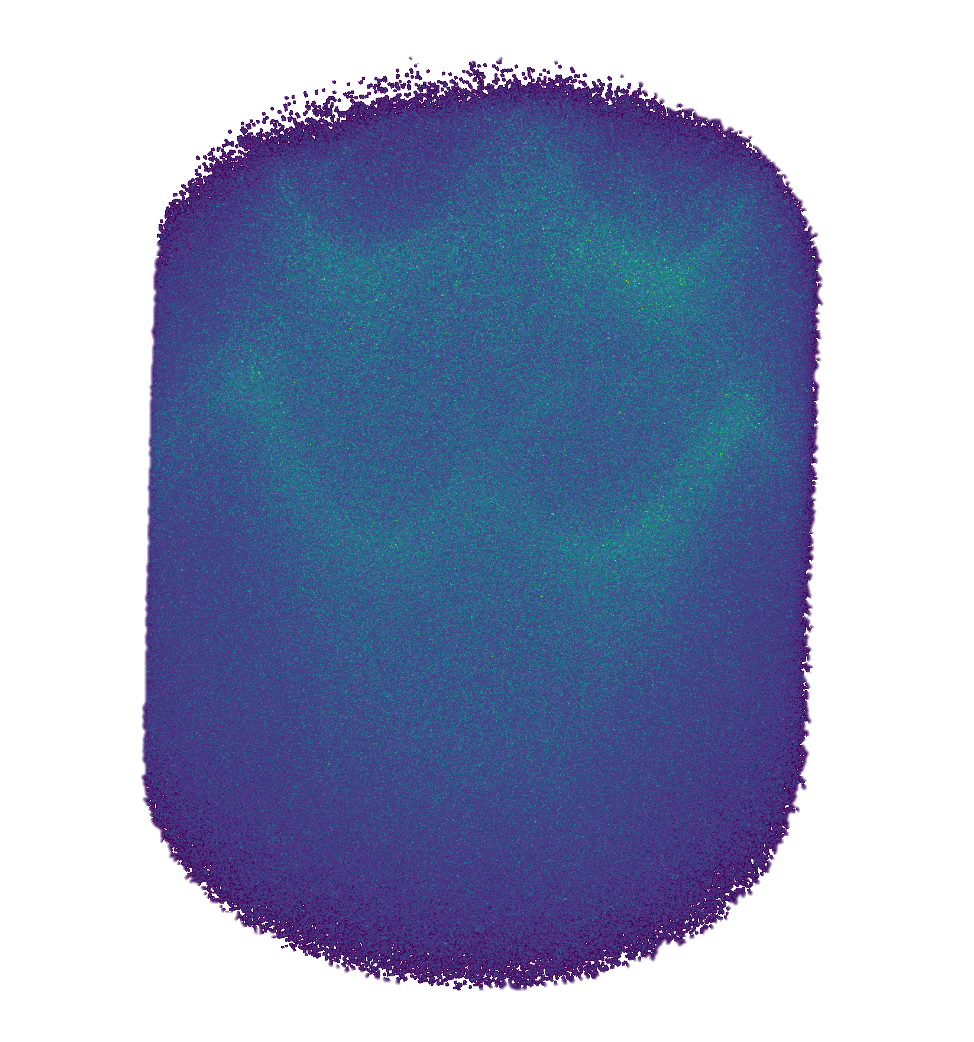
\includegraphics[width=1\linewidth]{images/3d_gr_ir_8M.png}
        \caption{$\gls{ncounts}=\num{8e6}$ corresponding to $\gls{total_time}=\qty{8}{min}$. The fine features of the data are not visible due to the low \gls{ncounts}.\todo[disable]{Do you really mean the ``rate'' (which you don't seem to specify) of the number of counts?}}
        \label{fig:3d-gr-ir-8M}
    \end{subfigure}
    \hfill
    \begin{subfigure}[t]{0.49\linewidth}
        \centering
        \includegraphics[width=1\linewidth]{images/3d_gr_ir_masked.png}
        \caption{$\gls{ncounts}=\num{1.86e8}$ corresponding to $\gls{total_time}=\qty{30}{hour}$. 2D images can be formed by slicing (or summing slices) along any of the axes, as depicted by the three lines.}
        \label{fig:3d-gr-ir-186M}
    \end{subfigure}
    \caption{3D images from the \gls{GrIr} dataset, with $\gls{ncounts}=\num{8e6}$ (left) \todo[disable]{insert ``(left)''} and \num{1.86e8} (right)\todo[disable]{insert ``(right)''}. The image is constructed by binning over the three detector axes $x$, $y$, $t_{\text{tof}}$, corresponding to the physical axes $k_x$, $k_y$, $E$. 2D images can be formed by slicing (or summing slices) along any of the axes, as depicted by the three lines (blue, green, purple) showing arbitrary summing sizes.}
    \label{fig:3d-gr-ir}
\end{figure}

\subsection{Generation of Noisy Realizations}\label{section:noisy-realizations}
In typical detection setups, generating noisy realizations $X$ of clean images $Y$ is limited by fixed integration windows. This means that the noise levels can only be varied in discrete steps, as multiples of the integration time, or by simulating noise post-capture. In contrast, the single-event stream enables us to obtain real and adjustable noisy realizations by selecting subsets of the varying electron counts \gls{ncounts} from the full dataset, without relying on simulated noise. This flexibility, by controlling the noise levels, has a major advantage in training and evaluating denoising algorithms on a large scale of noise levels.

The noisy image $X$ can be generated by taking a \gls{ncounts} subset of the complete dataset and then binned to form independent 3D images. For example, taking non-overlapping subsets of \gls{ncounts} being \num{e6} from the \gls{GrIr} dataset, we can generate \num{186} noisy realizations. The images can then be assumed to be formed with an \gls{iid} stochastic process, as the underlying data generation process is assumed \gls{iid} (\cref{section:photoelectron-counting-stats}). This assumption is discussed in more detail in \cref{ch:deep_learning} as it has important implications for training machine learning models. It should be noted that even for non-overlapping subsets, this assumption is only valid for short time scales, as the \gls{FEL} light source is generally not stable over extended acquisition periods, and other factors such as sample degradation, temperature deviations, etc., could break this assumption.

\todo[disable]{If you have a specif number here, I guess you mean also a specific data set. Which one is it? Due to this number, I guess \gls{GrIr}. And why 186? This looks like total number of counts divided by $10^6$, so you have data sets non-overlapping in time? Please make this clear in the text.}

\begin{table}[h!]
    \centering
    \resizebox{0.6\textwidth}{!}
        {%
        \begin{tabular}{lrrrc}
            \toprule
            \gls{ncounts} & Average Counts & $T$ [h] & Number of \\
            & Per Voxel & & Subsets \\
            \midrule
            \num{1e6} & \num{5.98e-3} & $\num{0.13}$ & 186 \\
            \num{2e6} & \num{1.22e-2} & $\num{0.28}$ & 93 \\
            \num{4e6} & \num{2.44e-2} & $\num{0.57}$ & 46 \\
            \num{8e6} & \num{4.89e-2} & $\num{1.23}$ & 23 \\
            \num{1.6e7} & \num{9.77e-2} & $\num{2.62}$ & 11 \\
            \num{3.2e7} & \num{2.00e-1} & $\num{5.32}$ & 5 \\
            \num{4.8e7} & \num{2.90e-1} & $\num{8.14}$ & 3 \\
            \num{9.6e7} & \num{5.84e-1} & $\num{16.07}$ & 1 \\
            \num{1.86e8} & \num{11.3e-1} & $\num{30.78}$ & 1 \\
            \bottomrule
        \end{tabular}
        }
    \caption{Summary of noisy realizations generated by varying number of electron counts \gls{ncounts} from the \gls{GrIr} dataset. The acquisition time \gls{total_time} is proportional to \gls{ncounts}, and \num{1.86e8} is used as the reference dataset.\todo[disable]{Just looking at this table and the text of Section 4.2.2, the $n$ column on the very left looks superfluous.}}
    \label{noisy-dataset-table}
\end{table}

To evaluate denoising performance across different noise levels, we generate a series of noisy realizations from the \gls{GrIr} dataset, each with a distinct total count, \gls{ncounts}. The total counts and average counts per voxel and acquisition time \gls{total_time} for each \gls{ncounts} is shown in \cref{noisy-dataset-table}. These realizations allow systematic assessment of the denoising algorithm performance under varying noise levels. Lower count realizations ($\gls{ncounts}<\num{1e7}$), corresponding to shorter \gls{total_time}, are of most interest to denoise. Successful denoising of such data (such as image seen in \cref{fig:3d-gr-ir-8M}) could significantly improve experimental efficiency, allowing the investigators to steer the experiment in the right direction, crucial in time-limited \glspl{beamtime}.

To balance coverage across a wide range of \gls{ncounts} from \numrange{1e6}{1.86e8} while limiting the number of generated realizations, we sampled \gls{ncounts} as successive multiples of prior values, allowing more focus on lower counts. This same approach is applied to generate noisy realizations in other datasets, ensuring comparability across a range of noise levels and acquisition times.

\section{Evaluation Criteria}
As described in the last section, a 3D image is constructed by binning over the three physical axes $k_x$, $k_y$, $E$ from different datasets. By slicing along these axes, different 2D images can be generated for analysis. We evaluate the \gls{BM3D} algorithm, with and without the Anscombe transform\footnote{This was discussed in detail in \cref{ch:denoising}.}, using the \gls{GrIr} dataset, which has the highest average counts of all datasets. Despite this, the average counts per voxel \todo[disable]{I assume ``average voxel intensity'' is supposed to be the same as ``average counts per voxel''? Please try to only use one way to describe / name one thing to avoid confusion.} is low (refer to last row of \cref{noisy-dataset-table})\todo[disable]{I assume this refers to the last colunm of the table, which is for the entire data set? Please make this more clear in the text.}, making a true, noise-free image unavailable. This limitation complicates the task of evaluating denoising performance, as standard metrics rely on comparison with such a noise-free reference.

Image quality assessment (IQA) is a field dedicated to measuring the objective and perceptual \todo[disable]{I don't understand what ``perpetual'' is supposed to mean here. A given image and a quality value derived from this image with a formula will never change over time.} quality of an image. Objective metrics such as \gls{PSNR}, \gls{SSIM}, \gls{MSE} and \gls{MSSSIM} require a reference image\footnote{The metric definitions can be accessed in \cref{sec:metrics}.}---the latent clean image---to compare the denoised image against. No-reference metrics also exist, such as natural image quality evaluator (NIQE). However, these metrics are designed for real-world images. Subjective metrics such as the mean opinion score (MOS) can also be used, but these require evaluations by a group of experts, which can be impractical \cite{eskiciogluImageQualityMeasures1995,linzhangFSIMFeatureSimilarity2011}.

\todo[disable]{I'd say the term ``latent'' is mostly linked to machine learning.}
\todo[disable]{What does make an image ``scientific''? Perpahps just drop the adjective.}
\todo[disable]{And would those even be objective?}

\begin{figure}
    \centering
    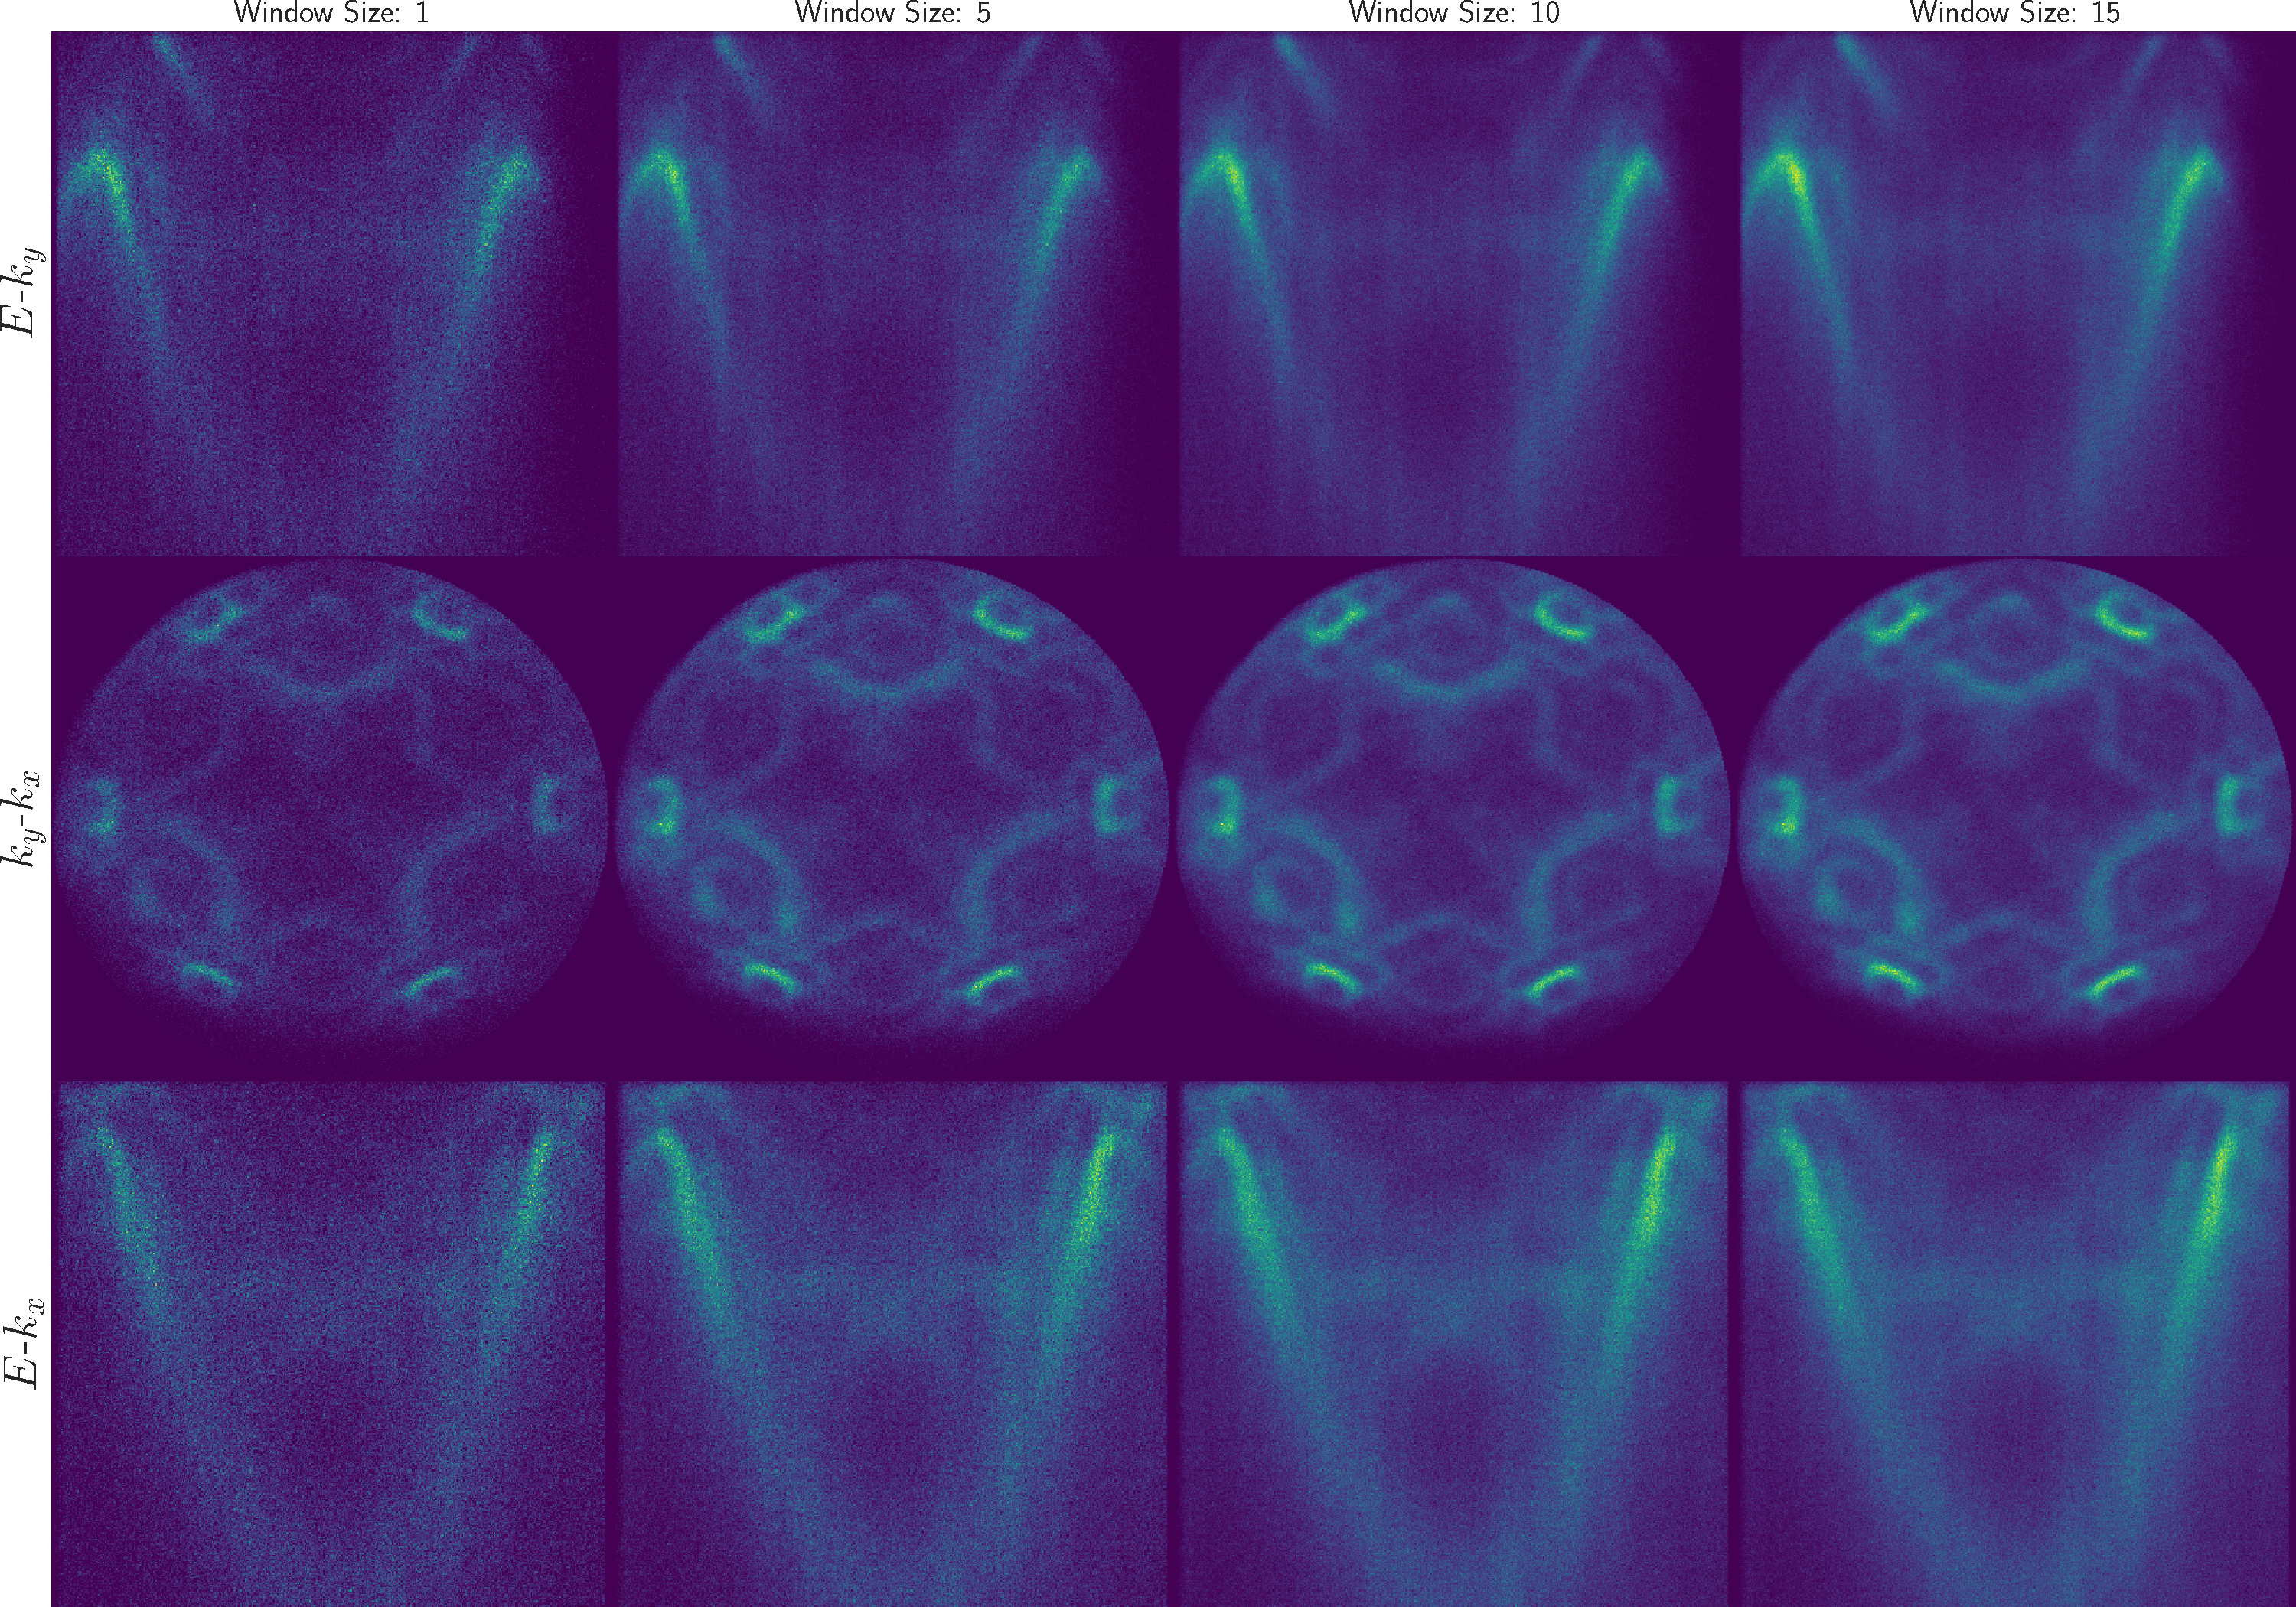
\includegraphics[width=0.8\linewidth]{images/slices.pdf}
    \caption{$E$, $k_y$, and $k_x$ slices at arbitrary positions of the \gls{GrIr} 3D dataset, showing the effect of summing with different  slice sizes \gls{winsize}. The left most column shows a single slice ($\gls{winsize}=1$) with significant noise, while subsequent columns show slice-summed images with $\gls{winsize}=\numlist{5;10;15}$. Increasing \gls{winsize} progressively reduces noise, at the cost of feature broadening (also referred to as blurring). This trade-off highlights the difficulty in obtaining a true, noise-free reference image even through averaging techniques.}
    \label{fig:slices}
\end{figure}

\todo[disable]{This broadeining is also often referred to as blurring.}

Given the low \gls{ncounts} in the datasets of interest, a possible method to create a higher quality reference image is to sum across neighboring slices. \cref{fig:slices} illustrates such a case, where noise is progressively reduced by summing across increasing slices (see \cref{fig:3d-gr-ir} for a 3D depiction of slice axis), at the cost of feature blurring. Even with a large slice summing, an ideal, noise-free reference image is not obtainable.

To address this, we assess metrics that are more resilient to noisy reference images. In \cref{sec:metric_comparison_experiment}, we compare the performance of different metrics (\gls{PSNR}, \gls{SSIM}, \gls{MSE} and \gls{MSSSIM}) for evaluating the denoising performance. Our findings suggest that the \gls{MSSSIM} metric is particularly well-suited for evaluating the denoising performance of images, when comparing against a noisy reference image. The \gls{MSSSIM} metric, conceived by \citeauthor{wangMultiscaleStructuralSimilarity2003} \cite{wangMultiscaleStructuralSimilarity2003}, extends SSIM by incorporating multiple scales. Furthermore, some randomly chosen estimated images are analyzed by an expert to provide a qualitative assessment of the denoising performance.

Given that the ideal denoising aims to produce distortion-free images, one free from artifacts and removing all unwanted signal, it makes sense to target structural similarity rather than relative intensity values against the reference. Hence, throughout this study, the images are normalized to the [\num{0}, \num{1}] range. This normalization ensures that comparisons focus on relative differences in image structures and features, rather than on absolute intensity values.

\section{Denoising MPES data with BM3D}
Let us start with  denoising the noisy realization with $\gls{ncounts}=\num{1.6e7}$ ($\gls{total_time}\approx\qty{2}{h}$) of the $k_y$-$k_x$ images shown in \cref{fig:slices}. This particular slice serves as a good reference due to its clear features. We use the Anscombe--\gls{BM3D}--Inverse Anscombe scheme described in \cref{fig:anscombe-bm3d}. 

\todo[disable]{You are not ``attempting to denoie'' you are ``denoising''.}
\todo[disable]{From $\gls{ncounts}=\num{1.6e7}$.}

\begin{figure}
    \centering
    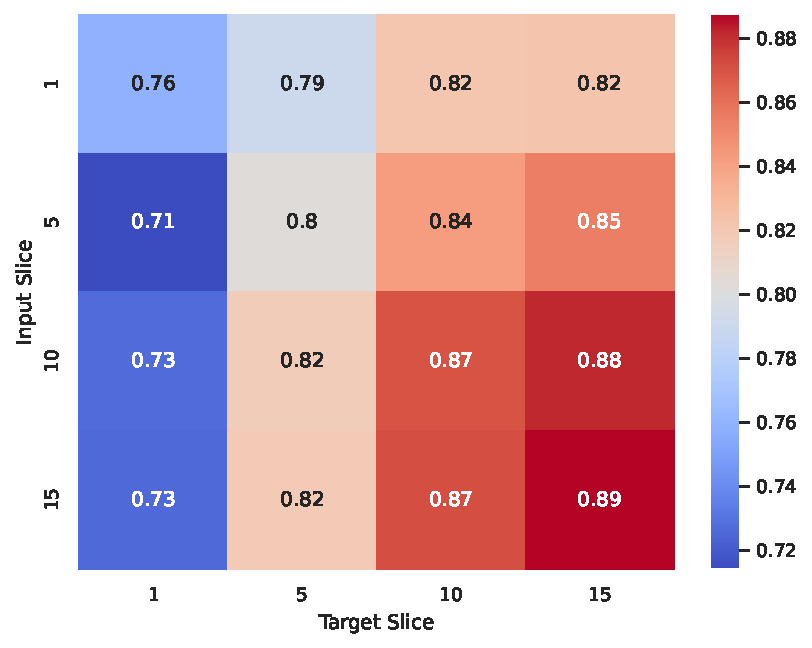
\includegraphics[width=0.5\linewidth]{images/confusion_matrix_msssim_window_avg.pdf}
    \todo[disable]{The color sheme seems somewhat counter-intuitive. Red is best?}
    \caption{Heatmap matrix \todo[disable]{I don't think that this should be called confusion matrix. This is a concept for classification problems.} showing the \gls{MSSSIM} values with different number of summed slices ($w$) for input and target images. The \gls{MSSSIM} (higher is better) is computed for the denoised images using the Anscombe-BM3D scheme. The matrix shows that using a larger $w$ for target image leads to better comparison of denoising.}
    \label{fig:confusion_matrix_msssim_window_avg}
\end{figure}

\begin{figure}
    \centering
    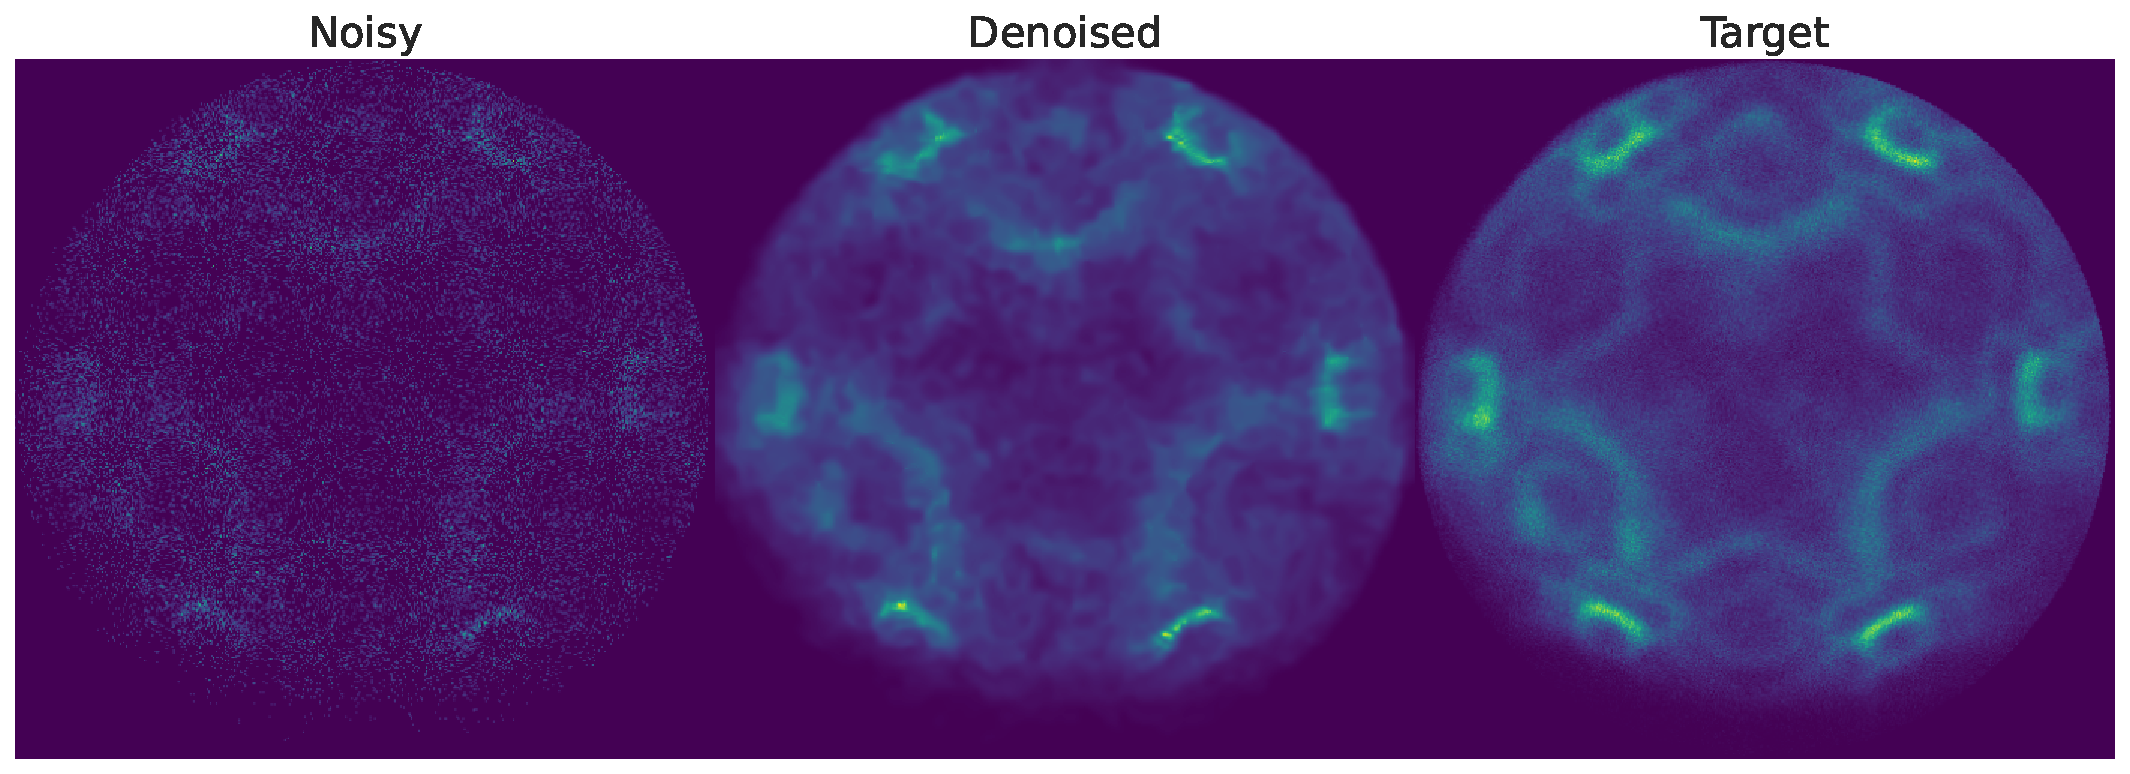
\includegraphics[width=1\linewidth]{images/noisy_denoised_ref_16M_avg_bm3d.pdf}
    \caption{Noisy, denoised, and target images. The noisy and target images are formed by summing slices with size $w=5$ and $w=15$ along the $E$ dimension, respectively.}
    \label{fig:noisy-denoised-ref-16M-avg-bm3d}
\end{figure}

We compare the effect of varying the slice summing size $w$ on the reported \gls{MSSSIM} score. Denoising the image with \gls{ncounts} of \num{1.6e7}, we compute the metric with $w = \numlist{1;5;10;15}$ (slice summing along the $E$ dimension) for all combinations of noisy and target (\gls{ncounts} of \num{1.86e8}) images. An example noisy ($w = 5$), denoised and target ($w=15$) set is shown in \cref{fig:noisy-denoised-ref-16M-avg-bm3d}. 

The matrix in \cref{fig:confusion_matrix_msssim_window_avg} shows that a larger $w$ yields a better comparison for denoising.  This is possibly because a larger $w$ reduces the noise in the target image, leading to a more accurate representation of a clean target image. However, it should also be addressed that the denoising quality is not uniform across all $w$ values, as the denoising algorithm has a parameter that, we will see in \cref{section:finding-optimal-sigma}, scales with the noise level. The results presented in \cref{fig:combined-metrics-comparison} with (a) $w=1$ and (b) $w=10$ support the idea that a larger $w$ is beneficial for denoising, as the reported metric values improve significantly with the increased $w$.


\todo[disable]{This is a bit confusion. You start by saying you do this for $w=5$ (noisy) and $w=15$ (target). Then you do it for $w = \numlist{1;5;10;15}$ for both noisy and target images. I would start with the latter and then just say that \cref{fig:noisy-denoised-ref-16M-avg-bm3d} shows this example $w=5$ (noisy) and $w=15$ (target)}
\todo[disable]{This assumes that the denoising has the same quality in all cases. This is not so clear since the denoising has a parameter that scales with the noise level and even though you keep $\gls{ncounts}$ constant, changing $w$ changes the noise strength (very visible in \cref{fig:slices})}

\subsection{Finding the Optimal Sigma}\label{section:finding-optimal-sigma}
\begin{figure}
    \centering
    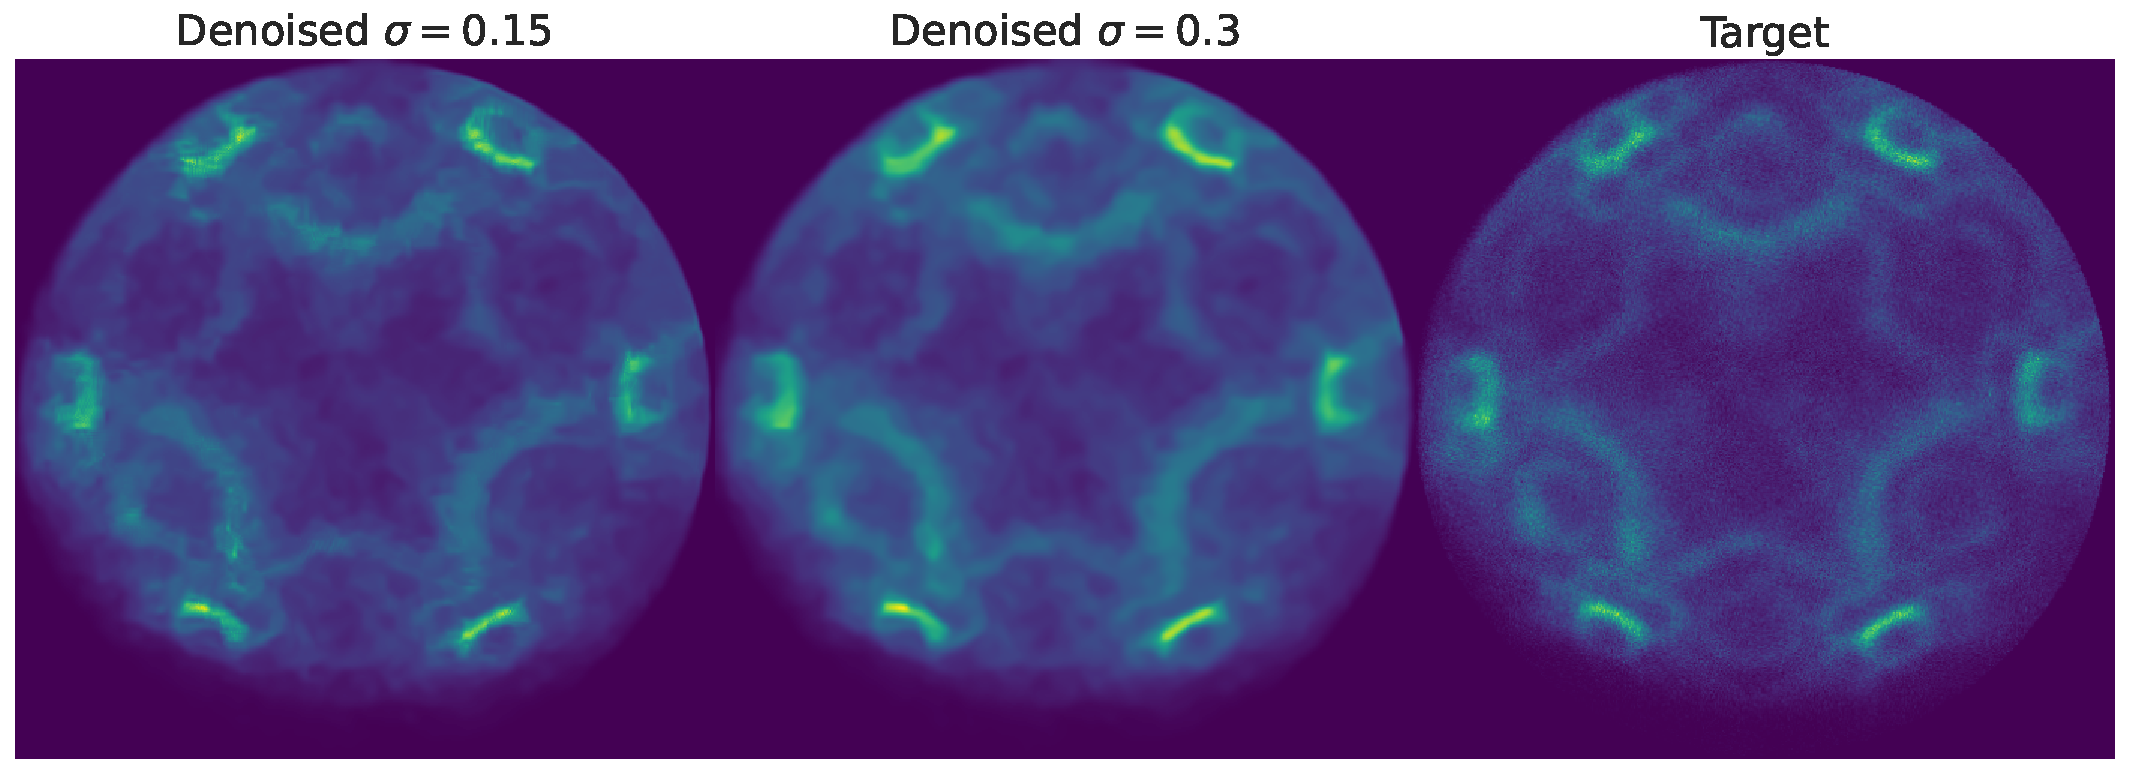
\includegraphics[width=1\linewidth]{images/denoised_optimal_sigma.pdf}
    \caption{(Left) Denoised image using the optimal $\sigma_{\text{oo}}=0.15$ (optimal value found for \num{1.6e7} counts from the hyperparameter search) (middle) denoised image with $\sigma_{\text{o}}=0.3$ (adjusted optimal value) and (right) the target image.}
    \label{fig:denoised-optimal-sigma}
\end{figure}
Till now, we only focused on a single electron count (\gls{ncounts}) and a fixed denoising parameter $\sigma$. However, considering that the noise decreases with increased electron counts (see \cref{section:law-of-large-numbers}), we would expect the required level of denoising to decrease accordingly.

\todo[disable]{This notation usually meant ``proprtional'', which indicates that here is linear relationship between both sides. Is this clear here from some BM3D properties?}

One way to find the optimal denoising strength would be to estimate the noise level and use that estimate as the $\sigma$ for denoising. This approach requires prior knowledge or assumptions about the noise distribution. Instead, it empirically finds the best parameters for denoising.

A different approach would be to perform an \todo[inline]{Why constrained?} optimization to find optimal $\sigma$ denoted $\sigma_{\text{oo}}$, such that an objective function, such as the \gls{MSSSIM} metric, is maximized\todo[inline]{Optimizing for \gls{MSSSIM} and then using \gls{MSSSIM} as quality measure is a bit dangerous and should at least be discussed a bit.}. For user defined parameters to an algorithm, this sort of optimization is known as a hyperparameter search\todo[inline]{Reference?}. 

\todo[disable]{Mention why you are not doing this.}

Finding the optimal parameter through an exhaustive grid search is the simplest method, but it is computationally expensive. We perform a hyperparameter search with \texttt{optuna}\footnote{\href{https://optuna.org/}{https://optuna.org/} see citation in acknowledgments.}\todo[inline]{I think there is also a paper to cite for Optuna.}, which uses Bayesian optimization to find the optimal hyperparameters.

The search is conducted \todo[inline]{Is this done for \cref{alg:bm3d} or \cref{alg:anscombe-bm3d}? Or both? I couldn't find this info in the text.} on a small set of \num{5} identical featured \todo[inline]{What does ``identical featured'' mean? Are this just two images that are very similar to the one in \cref{fig:noisy-denoised-ref-16M-avg-bm3d}? How is this similarity measured? In the ``eyeball'' metric?} images (same slice), featuring the same characteristics as shown in \cref{fig:noisy-denoised-ref-16M-avg-bm3d}, slice summed with $\gls{winsize} = \num{10}$\todo[inline]{Why $w=10$?} across the count range of \numrange{1e6}{4.8e7}. The search is conducted over \num{50} trials for each \gls{ncounts} and each image. The optimization maximizes \gls{MSSSIM} score by adjusting the denoising parameter $\sigma$, which is constrained between \numrange{0}{5} to prevent the disappearance of features, as higher values can lead to significant loss of detail\todo[inline]{And negative values of $\sigma$ are impossible.}.

\begin{figure}
    \centering
    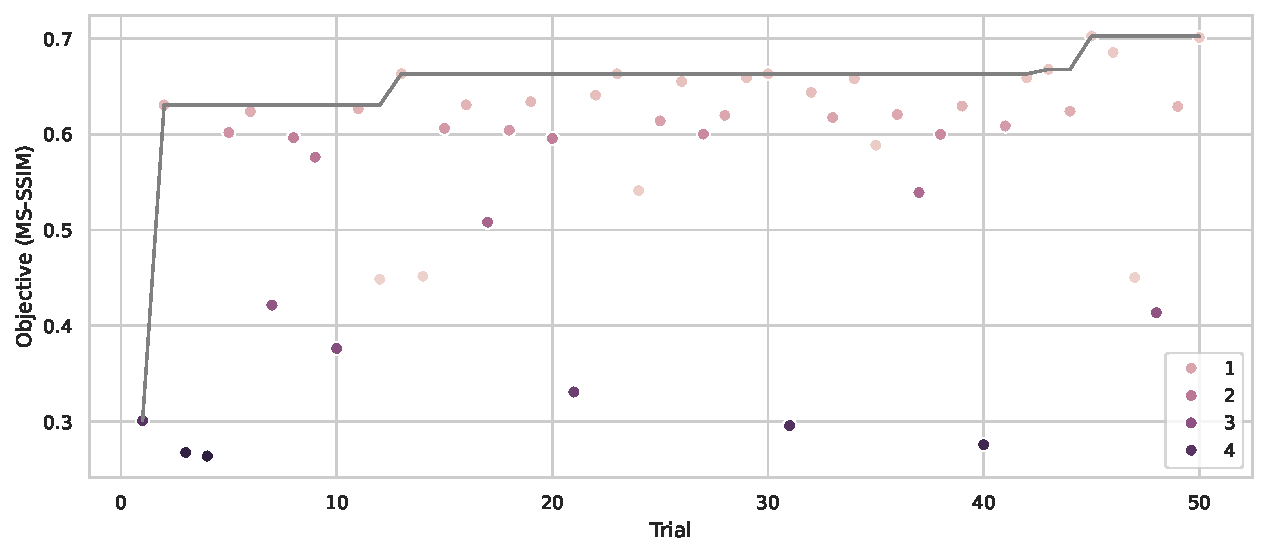
\includegraphics[width=\textwidth]{images/optimization_against_trial.pdf}
    \caption{Example optimization study to find optimal BM3D hyperparameter $\sigma$: The plot shows how the optimization takes course over the trials using \gls{MSSSIM} score, which serves as the objective in the hyperparameter optimization. The cumulative maximum \gls{MSSSIM} score achieved up to each trial is shown as a gray line. The color of the scatter points represent the sigma parameter for each trial, with larger and darker points indicating higher values of sigma, showing that most time is spent near the optimal sigma.}
    \label{fig:optimization-against-trial}
\end{figure}

The optimization process for a single image (from \gls{ncounts} of \num{2e6}) is illustrated in \cref{fig:optimization-against-trial}. This figure shows the progression of the optimization process across trials. The Bayesian optimization efficiently explores the parameter space, with most trials focusing near the optimal $\sigma$ value, to maximize the \gls{MSSSIM} score.

The results in \cref{fig:hyperparameter-averaged-10-images} corroborate the hypothesis that the optimal $\sigma$ for denoising decreases with increasing electron counts, a linearly decreasing trend.




\begin{figure}
    \centering
    \begin{subfigure}[t]{0.49\linewidth}
        \centering
        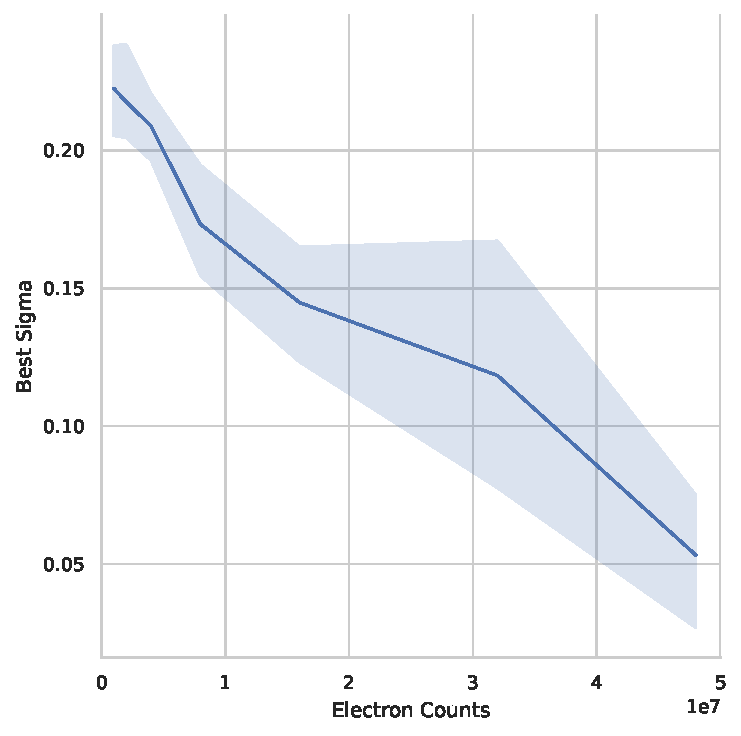
\includegraphics[width=\linewidth]{images/hyperparameter_sigma_averaged_10_images.pdf}
        \caption{Optimal sigma value $\sigma_{\text{oo}}$ as a function \gls{ncounts}, showing how the optimal denoising decreases with increasing electron count.}
        \label{fig:hyperparameter-sigma-averaged-10-images}
    \end{subfigure}
    \hfill
    \begin{subfigure}[t]{0.49\linewidth}
        \centering
        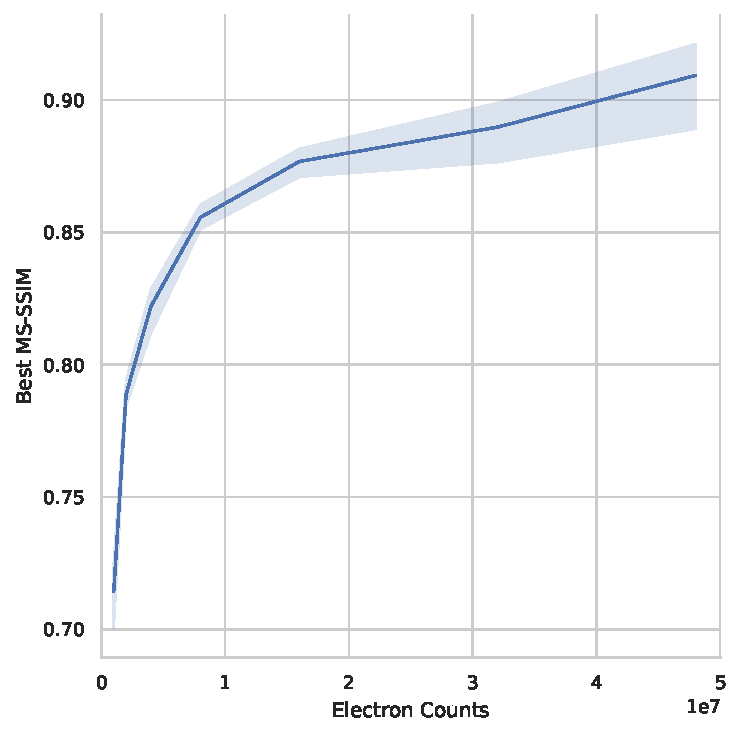
\includegraphics[width=\linewidth]{images/hyperparameter_msssim_averaged_10_images.pdf}
        \caption{\gls{MSSSIM} score as a function \gls{ncounts}, indicating that the denoising performance does not scale linearly with \gls{ncounts}, even when using optimal parameters.}
        \label{fig:hyperparameter-msssim-averaged-10-images}
    \end{subfigure}
    \caption{The plots show the relationship between electron counts \gls{ncounts} and \gls{BM3D} denoising performance. (Left) The optimal value of the denoising parameter, sigma $\sigma_{\text{oo}}$, and (right) the corresponding \gls{MSSSIM} score, which serves as the optimization objective. These results were obtained from \num{50} trials for each noisy image (slice summed with size $w=10$ across $E$), with the optimization focused on maximizing the \gls{MSSSIM} score by adjusting $\sigma$. The \num{95}\% confidence interval is shown, computed over \num{5} images for each count.}
    \todo[inline]{I don't fully understand where you get the standard deviation from. Is the area around the curve even the standard deviation? You don't actually say what this is supposed to show. Please elaborate more in the text what data exactly you use (in particular how many of which type). There seem to be two target images, but I don't see any mention on how many noisy images you use per selected count value.}
    \label{fig:hyperparameter-averaged-10-images}
\end{figure}

While using \gls{MSSSIM} as the objective function for optimization is good at showing the denoising performance improvement, it leads to more cautious results (low $\sigma_{\text{oo}}$ values) as those fare better against the target, which has the relevant features but is also noisy. To counter that, we scale the optimum $\sigma_{\text{oo}}$ values by a factor of 2 to get a more aggressive denoising and denote that as $\sigma_{\text{o}}$ and use this for denoising. A comparison of the denoised image using the adjusted optimal $\sigma_{\text{o}}$ and the optimal $\sigma_{\text{oo}}$ is shown in \cref{fig:denoised-optimal-sigma}.

The denoising performance below \num{4e6} \todo[inline]{Does ``below'' mean ``lower equal''? \num{4e6} doesn't look so bad to me, but the text seem to indicate that both results are poor.} is poor, with or without the optimal value $\sigma_{\text{oo}}$, even though the \gls{MSSSIM} reports high values. \cref{fig:noisy-denoised-ref-2M-avg-bm3d} and \cref{fig:noisy-denoised-ref-4M-avg-bm3d} show the denoised images for \num{2e6} and \num{4e6} counts, with an average count of \num{0.14} and \num{0.27} \todo[inline]{This doesn't seem to fit to the values in \cref{noisy-dataset-table}. Do you perhaps mean total count instead of average count? Or average total count? Where I'm not sure what you are averaging over.} in the noisy image, respectively, whereas the average count in target image is \num{12.9}. It can be seen that the perceptual \todo[inline]{Again, I don't understand ``perpetual'' in this context.} quality of the denoised images is poor, with the features not being well-preserved. This highlights that \gls{BM3D} is not well suited for denoising such low-count images.

\begin{figure}
    \centering

    \begin{subfigure}[b]{1\linewidth}
        \centering
        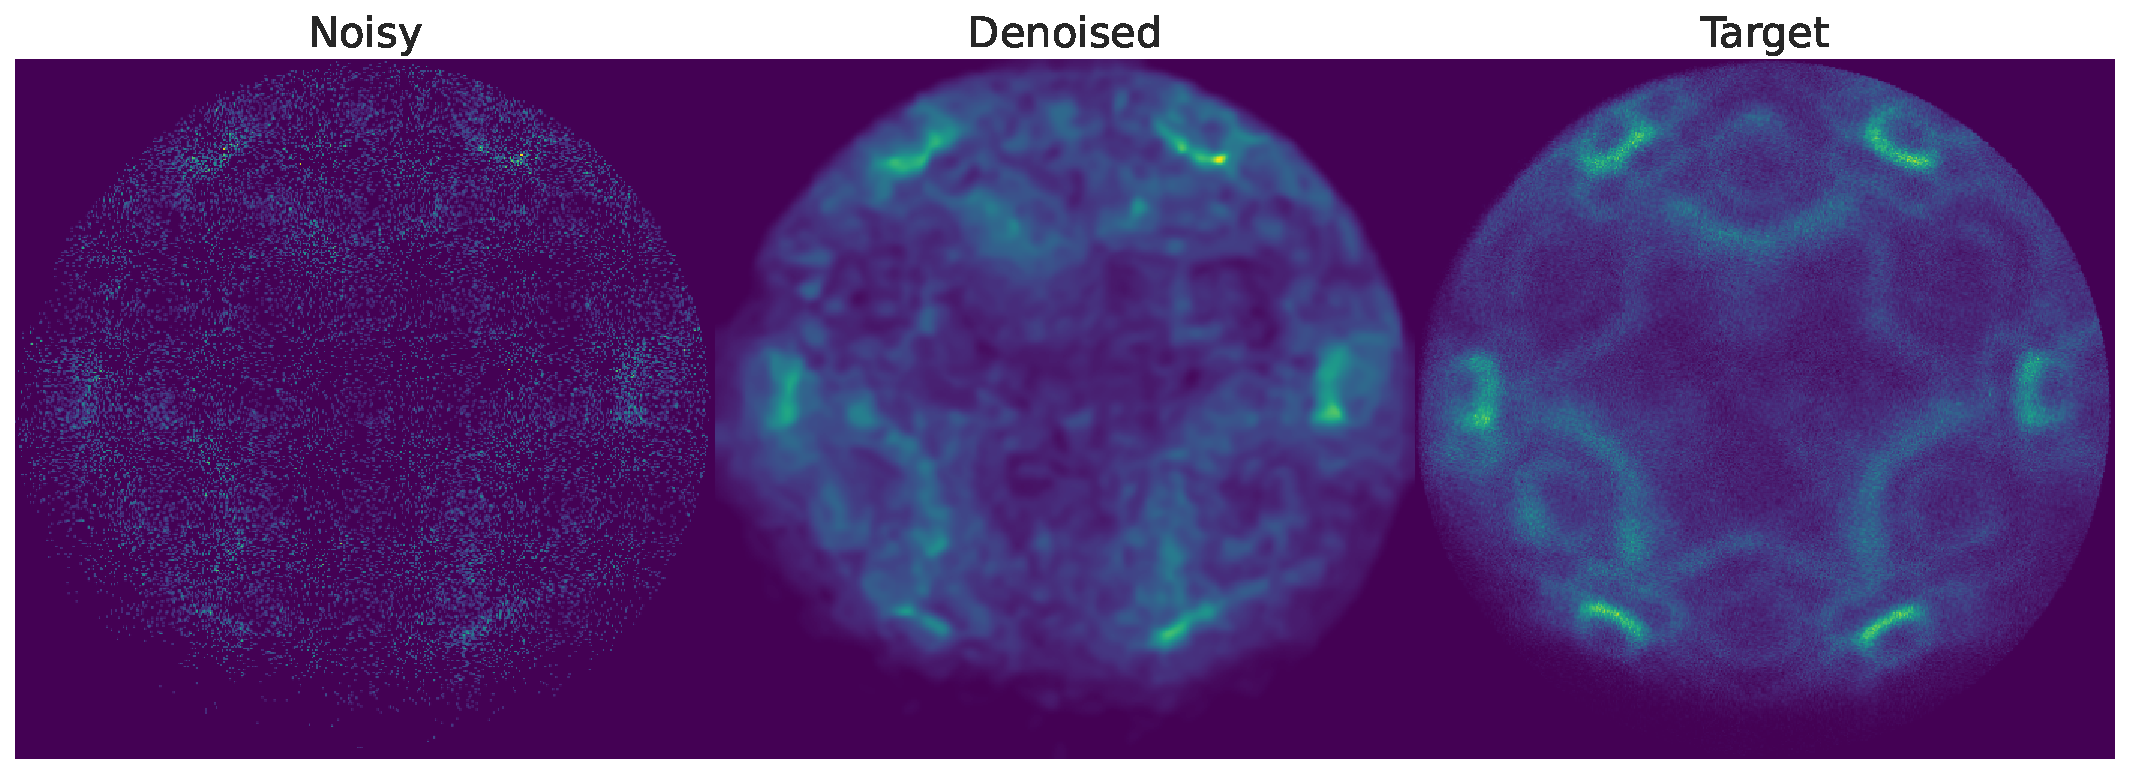
\includegraphics[width=1\linewidth]{images/noisy_denoised_ref_2M_avg_bm3d.pdf}
        \caption{Dataset with $\gls{ncounts}=\num{2e6}$. The denoising performance is quite poor, even with the adjusted optimal $\sigma_{\text{o}}\approx0.4$.}
        \label{fig:noisy-denoised-ref-2M-avg-bm3d}
    \end{subfigure}

    \begin{subfigure}[b]{1\linewidth}
        \centering
        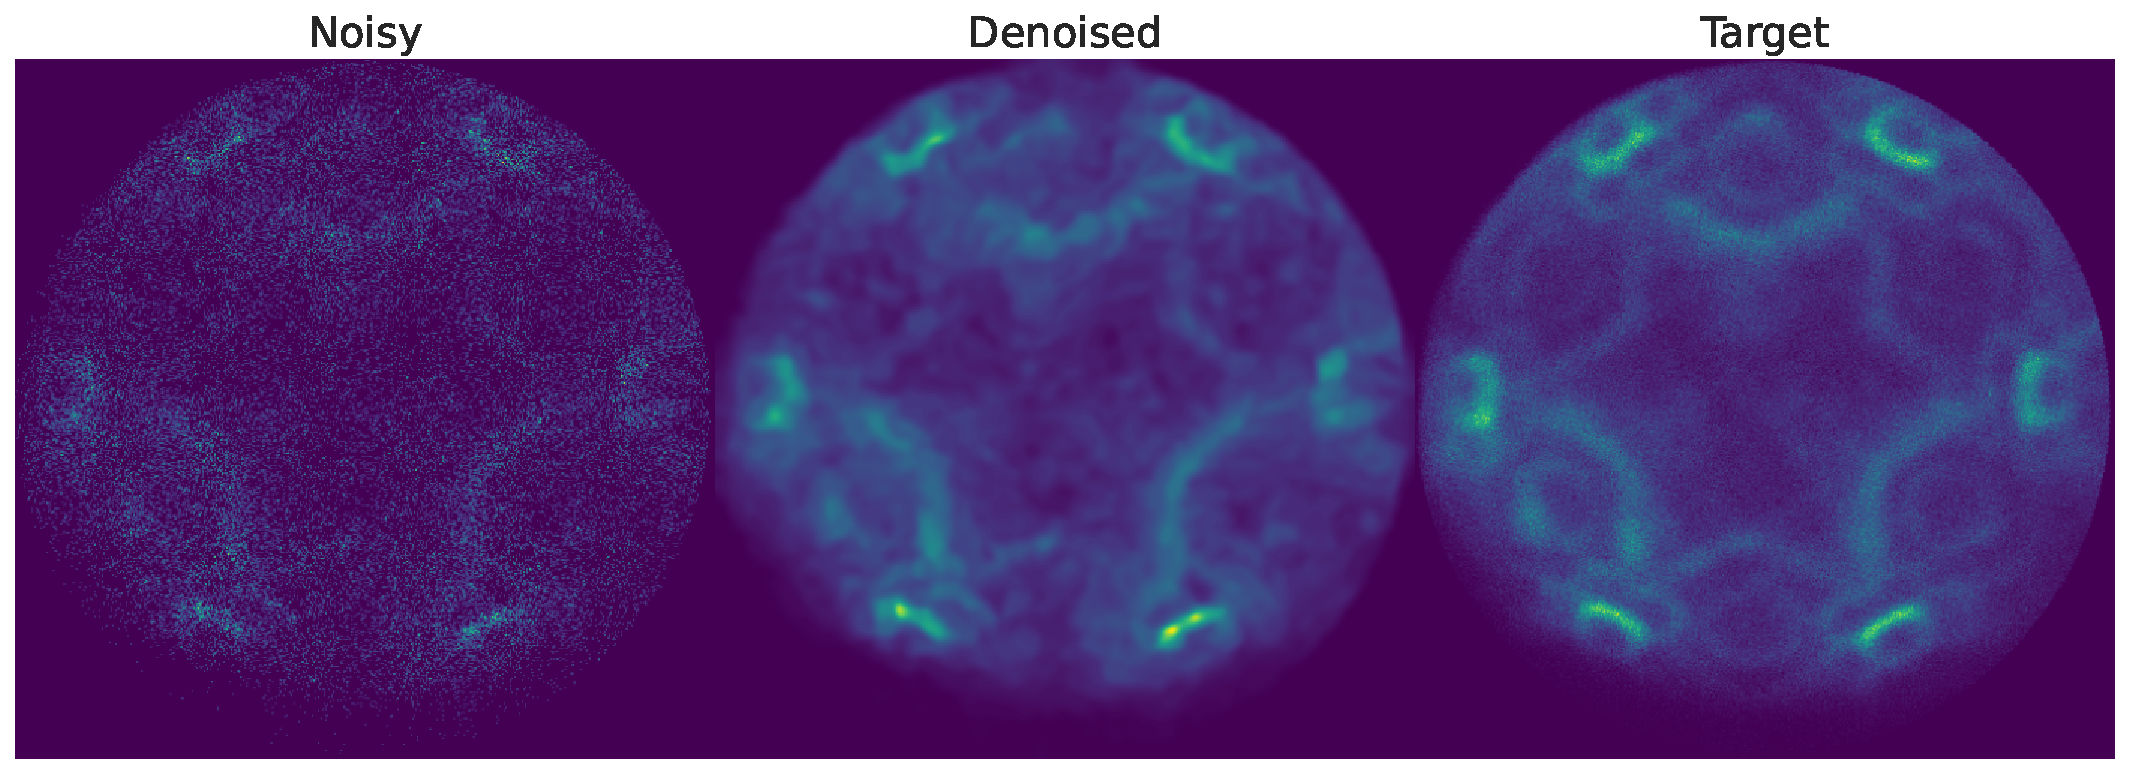
\includegraphics[width=1\linewidth]{images/noisy_denoised_ref_4M_avg_bm3d.pdf}
        \caption{Dataset with $\gls{ncounts}=\num{4e6}$. The denoising performance leaves room for improvement, using the adjusted optimal $\sigma_{\text{o}}\approx0.4$.}
        \todo[inline]{The number of counts is twice of the example in the first row, but $\sigma_{\text{o}}$ is the same?}
        \label{fig:noisy-denoised-ref-4M-avg-bm3d}
    \end{subfigure}

    \begin{subfigure}[b]{1\linewidth}
        \centering
        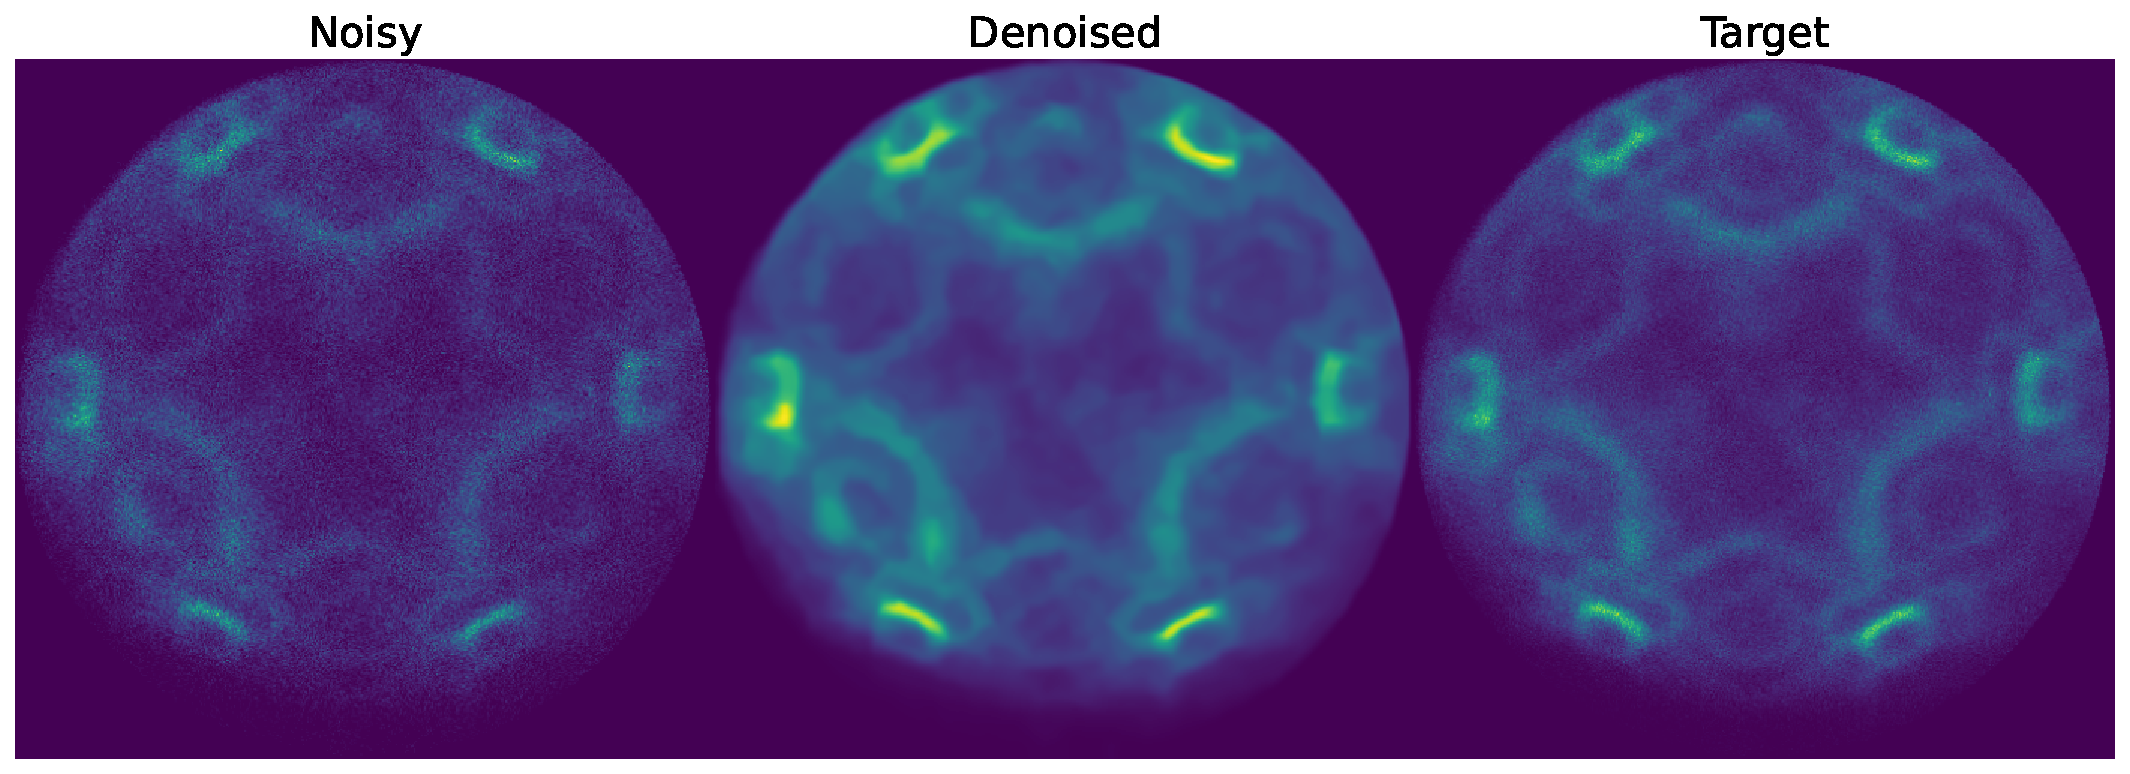
\includegraphics[width=1\linewidth]{images/noisy_denoised_ref_48M_avg_bm3d.pdf}
        \caption{Dataset with $\gls{ncounts}=\num{4.8e7}$. At this \gls{ncounts}, \gls{MSSSIM} reports lower values for the denoised images compared to the noisy images, even though the denoised image features are well-preserved.}
        \todo[inline]{What is $\sigma_{\text{o}}$ here? You mention it in both rows above.}
        \label{fig:noisy-denoised-ref-48M-avg-bm3d}
    \end{subfigure}

    \caption{Comparison of noisy, denoised, and target images for $\gls{ncounts}=$\numlist{2e6;4e6;4.8e7}, where the noisy and target images were formed using with $\gls{winsize}=\num{10}$ over \gls{E} to form \gls{kx}-\gls{ky} images. The \gls{BM3D} algorithm with Anscombe transform was used for denoising.}
    \label{fig:combined-noisy-denoised}
\end{figure}

\subsection{Varying Total Counts}
We now evaluate the denoising performance of \cref{alg:bm3d} (\gls{BM3D} without Anscombe) and \cref{alg:anscombe-bm3d} (\gls{BM3D} with Anscombe), using the optimal $\sigma_{\text{o}}$ values determined through the hyperparameter search. A total of \num{1847} images \todo[inline]{How many per $\gls{ncounts}$ value?} were extracted from two separate noisy realizations of \gls{ncounts} of \numlist{1e6;2e6;4e6;8e6;1.6e7;3.2e7;4.8e7}. These are slice summed with $\gls{winsize}=10$ for both the noisy and target images. 

As before, the \gls{MSSSIM} metric is used, with the baseline computed using the noisy images. Averaging over the large amount of images at varied counts gives us a robust estimate of the denoising performance. Using statistical bootstrapping\todo[inline]{Please elaborate what you mean with ``statistical bootstrapping''. Is this more than just computing this for different samples and then computing the mean and confidence interval from those values?}, where the estimate is computed over multiple resamples of the data, we can also estimate the \num{95}\% confidence interval of the \gls{MSSSIM} metric\todo[inline]{Does this mean these ``bands'' in the figure show the \num{95}\% confidence interval? This needs to be mentioned in the figure caption.}.

As shown in \cref{fig:bm3d-msssim}, there is a noticeable improvement in image quality with counts up to $\gls{ncounts}=\num{4e7}$, with \gls{MSSSIM} values increasing from \num{0.6} to \num{0.83}. Beyond this count, the metric starts reporting lower values for denoised results, whereas visual inspection reveals that the denoised images contain similar information as the target, smoother with preserved features. We can see this in \cref{fig:noisy-denoised-ref-48M-avg-bm3d}, where the denoised image has a lower \gls{MSSSIM} value compared to the noisy image, but the features are well-preserved. This necessitates the need for higher quality target images for better evaluation.\todo[inline]{In particular, this also shows that \gls{MSSSIM} has be interpreted carefully, but we just don't have a better measure.}

\begin{figure}
    \centering
    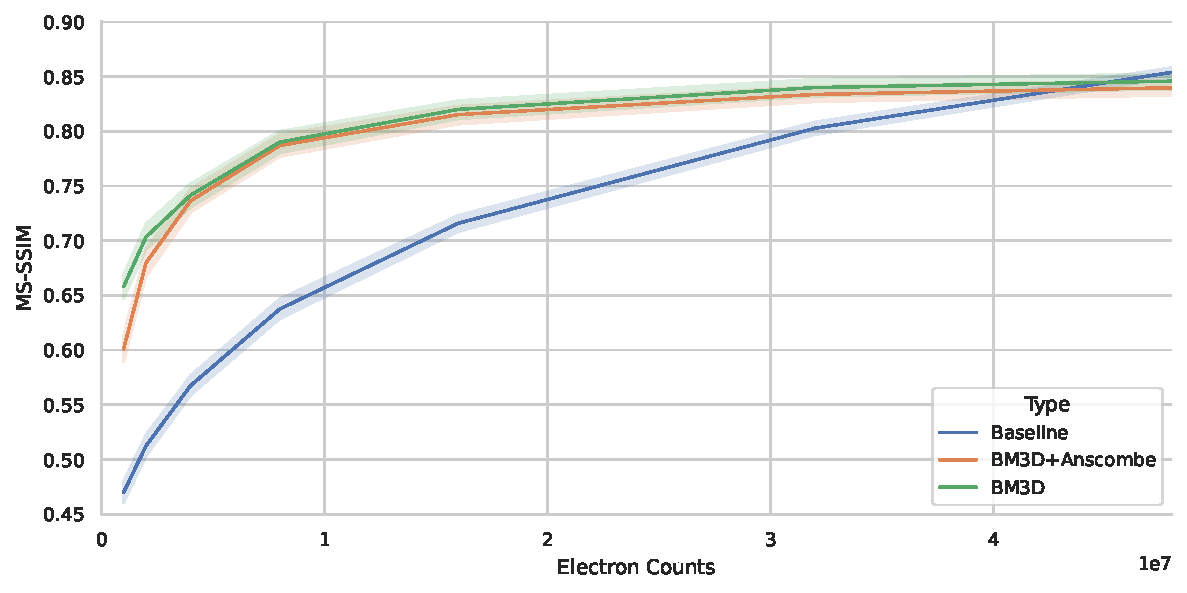
\includegraphics[width=1\linewidth]{images/bm3d_msssim.pdf}
    \caption{Denoising performance of the \gls{BM3D} algorithm, with and without the Anscombe transformation. The optimal $\sigma_{\text{o}}$ values determined through the hyperparameter search are used\todo[inline]{As I asked above, where the parameters computed for \cref{alg:bm3d} and \cref{alg:anscombe-bm3d} separately? Or just for one and also applied to the other?}. The images are slice summed with $\gls{winsize}=10$ slices for both the noisy and target images. The baseline metric is computed using the noisy image as input.}
    \label{fig:bm3d-msssim}
\end{figure}


The most notable finding is that the application of the \gls{VST} leads to a slightly worse performance (\cref{fig:bm3d-msssim} orange vs.\ green lines)\todo[inline]{It may also show that the \gls{MSSSIM} is not accurate enough. What does the ``eyaball'' metric say? A figure with example results could be helpful here.}, despite the expectation that it would enhance denoising performance for Poissonian noise. In previous work by \citeauthor{makitaloOptimalInversionAnscombe2011}, the authors demonstrated that applying the Anscombe transform indeed improves denoising performance. This strongly suggests that the noise statistics in the image deviate from a Poisson distribution. One reason is the slice summing used to form the images\todo[inline]{The sum of two independent Poisson random variables is Poisson.}, that might have altered the noise statistics. The other obvious reason is that the electron count statistics forming the images are not Poissonian. This shall be the topic of the next chapter. 
